\chapter{\ifproject%
\ifenglish Project Structure and Methodology\else โครงสร้างและขั้นตอนการทำงาน\fi
\else%
\ifenglish Project Structure\else โครงสร้างของโครงงาน\fi
\fi
}

\makeatletter

% \renewcommand\section{\@startsection {section}{1}{\z@}%
%                                    {13.5ex \@plus -1ex \@minus -.2ex}%
%                                    {2.3ex \@plus.2ex}%
%                                    {\normalfont\large\bfseries}}

\makeatother
%\vspace{2ex}
% \titleformat{\section}{\normalfont\bfseries}{\thesection}{1em}{}
% \titlespacing*{\section}{0pt}{10ex}{0pt}

\section{โครงสร้างโดยรวมของโครงงาน (Project Overview) }
\begin{mypara}
    \indent โครงงานนี้เป็นระบบสนับสนุนการตัดสินใจสำหรับการวางแผนระบบขนส่งสาธารณะ 
    โดยจะจัดทำเป็นเว็บแอพลิเคชั่นสำหรับการจำลอง และมีการสรุปผลลัพธ์ที่ได้จากการจำลองในรูปแบบทางสถิติ
    ซึ่งในการทำงานของระบบนี้จะมี 4 องค์ประกอบหลักดังนี้ที่ประกอบกันเป็นระบบเดียวกัน ดังภาพ \ref{fig:overview}  
\end{mypara}


\begin{figure}[H]
    \centering
    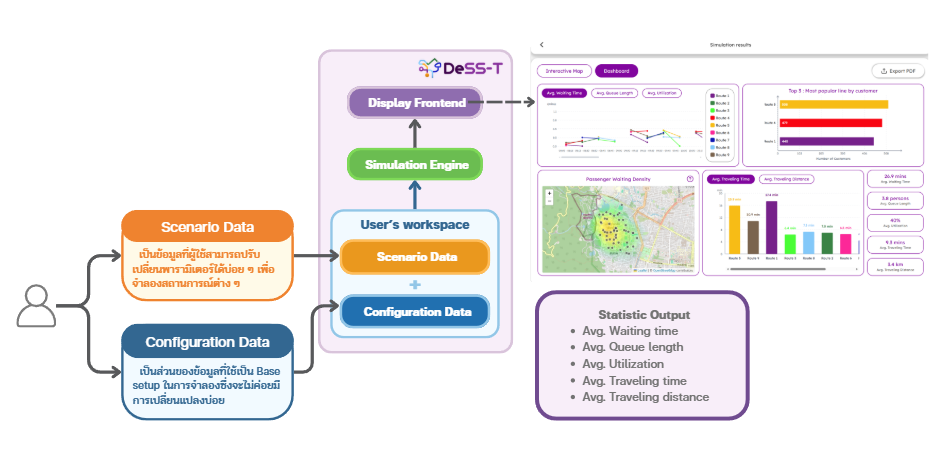
\includegraphics[width=\textwidth,height=0.9\textheight,keepaspectratio]{overview.png}
    \caption{แผนภาพโดยรวมของโครงงาน}
    \label{fig:overview}
\end{figure}

\subsection{ข้อมูลสถานการณ์ (Scenario data)}
\begin{mypara}
  \indent เป็นข้อมูลที่ผู้ใช้สามารถปรับเปลี่ยนพารามิเตอร์ได้บ่อย ๆ เพื่อจำลองสถานการณ์ต่าง ๆ 
  สำหรับการเปรียบเทียบและวางแผน ประกอบด้วย เส้นทางการให้บริการของรถในแต่ละสายบริการ 
  ตารางเวลาการออกรถ ช่วงเวลาที่ต้องการดูผลการจําลอง ข้อมูลของรถซึ่งมี 
  ความจุผู้โดยสารระยะทางที่สามารถวิ่งได้สูงสุด ความเร็วในการวิ่ง
\end{mypara}
\subsection{ข้อมูลการกำหนดค่า (Configuration data)}
\begin{mypara}
  \indent เป็นส่วนของข้อมูลที่ใช้เป็นพื้นฐานในการจำลองซึ่งจะไม่ค่อยมีการเปลี่ยนแปลงบ่อย 
  ได้แก่ ข้อมูลช่วงระยะห่างของเวลาที่ผู้โดยสารแต่ละคนมาถึงที่สถานี ข้อมูลของจำนวนผู้โดยสารที่ลงจากรถในแต่ละสถานี 
  และข้อมูลที่เกี่ยวข้องกับสถานีซึ่งจะเก็บในรูปแบบของ network model ซึ่งจะมี 
  node เป็นรายชื่อสถานี และ มี edge เป็นระยะทางระหว่างแต่ละสถานี
  \end{mypara}
\subsection{ส่วนการจำลอง (Simulation Component)}
\begin{mypara}
  \indent เป็นส่วนที่ทำหน้าที่ในการจำลองระบบขนส่งสาธารณะตามข้อมูลที่ได้รับจากส่วน scenario data 
  และ configuration data ซึ่งจะใช้เทคนิคการจำลองแบบเหตุการณ์ไม่ต่อเนื่อง (discrete-event simulation) และเทคนิคการจำลองแบบสุ่มเชิงสถิติ (stochastic simulation) 
  ในการจำลองระบบขนส่งสาธารณะ 
\end{mypara}
\subsection{ผลลัพธ์ (Output)}
\begin{mypara}
  \indent เป็นส่วนที่แสดงผลลัพธ์ที่ได้จากการจำลอง โดยจะมีข้อมูล เวลาการรอเฉลี่ยของผู้โดยสาร (average waiting time) ระยะแถวคอยเฉลี่ยของผู้โดยสาร (average queue length) 
  ระยะทางเฉลี่ยต่อแถวการเดินทาง (average traveling distance) ระยะเวลาระหว่างการเดินทาง (average travel time) และอัตราการใช้งานของรถและสถานี (average utilization)
  ซึ่งจะมีข้อมูลแสดงทั้งข้อมูลรวมทุกสถานีในช่วงระยะเวลาการจำลองทั้งหมด ภาพรวมการเดินรถในรูปแบบแผนที่โต้ตอบ (interactive map) พร้อมข้อมูลรายละเอียดของแต่ละสถานีแยกกันในแต่ละช่วงเวลาย่อย (time slots) 
  รวมถึงจะมีกระดานสรุปข้อมูล (dashboard) สำหรับแสดงผลลัพธ์ในรูปแบบกราฟเพื่อให้ผู้ใช้สามารถวิเคราะห์ข้อมูลได้ง่ายขึ้น 
\end{mypara}
\section{ขั้นตอนการทำงานของระบบ (System Workflow)}
\begin{mypara}
    \indent โครงงานนี้ทำงานโดยนำข้อมูลสถานการณ์จากผู้ใช้ (scenario data) มาจำลองระบบขนส่งสาธารณะ 
    โดยอ้างอิงจากข้อมูลการกำหนดค่า (configuration data) ซึ่งประกอบด้วยข้อมูลหลายประเภท 
    โดยบางส่วนจะถูกนำไปสร้างเป็น ฟังก์ชันการแจกแจง (distribution function) เพื่อใช้ในการสุ่มพฤติกรรมของผู้โดยสาร 
    ขณะที่ข้อมูลอีกส่วนจะถูกนำมาใช้โดยตรง ใน ส่วนการจำลอง ซึ่งจะประมวลผลด้วย
    เทคนิคการจำลองแบบเหตุการณ์ไม่ต่อเนื่อง (discrete-event simulation) และเทคนิคการจำลองแบบสุ่มเชิงสถิติ (stochastic simulation) 
    เพื่อสร้างผลลัพธ์เชิงสถิติที่สะท้อนประสิทธิภาพของระบบขนส่งสาธารณะมาแสดงผลในส่วน output
\end{mypara}
\subsection{การทำงานของข้อมูลการกำหนดค่าในระบบ (Configuration flow)}
\begin{mypara}
  \indent ข้อมูลการกำหนดค่า (configuration data) ประกอบด้วยข้อมูลที่รับมาจากผู้ใช้ทั้งหมด 3 ประเภท ได้แก่ ข้อมูลขอบเขตพื้นที่ที่จะทำการจำลอง (map area configuration) 
    ข้อมูลช่วงระยะห่างของเวลาที่ผู้โดยสารแต่ละคนมาถึงที่สถานี (interarrival data) และข้อมูลของจำนวนผู้โดยสารที่ลงจากรถในแต่ละสถานี (alighting data) โดยทั้งหมดจะผ่านกระบวนการดังนี้
\begin{itemize}
    \item ข้อมูลขอบเขตพื้นที่ที่จะทำการจำลอง (map area configuration) ส่วนนี้จะรับข้อมูลได้ 2 รูปแบบคือ รหัสพื้นที่ (area code) หรือ พิกัดของพื้นที่ (geographical coordinates) โดยจะนำมาเป็นคำหลัก (keyword) ในการค้นหาข้อมูลในฐานข้อมูล Openstreetmap ซึ่งจะถูกนำมาใช้ในการสร้าง network model ซึ่งจะมี node เป็นรายชื่อสถานี และ มี edge เป็นระยะทางระหว่างแต่ละสถานี
    \item ข้อมูลช่วงระยะห่างของเวลาที่ผู้โดยสารแต่ละคนมาถึงที่สถานี (interarrival data) และข้อมูลของจำนวนผู้โดยสารที่ลงจากรถในแต่ละสถานี (alighting data) จะนำเข้าสู่ระบบในรูปแบบไฟล์สกุล .xlsx ซึ่งระบบจะทำการอ่านข้อมูลจากไฟล์
    และจะถูกนำมาใช้ในการสร้างฟังก์ชันการแจกแจง (distribution function) 
\end{itemize}
  \indent หลังจากข้อมูลแต่ละส่วนผ่านกระบวนการข้างต้นแล้ว ทั้งหมดจะถูกรวมกันเป็นข้อมูลการกำหนดค่า (configuration data) ดังในภาพ \ref{fig:configuration_flow} 
\end{mypara}

\begin{figure}[H]
    \centering
  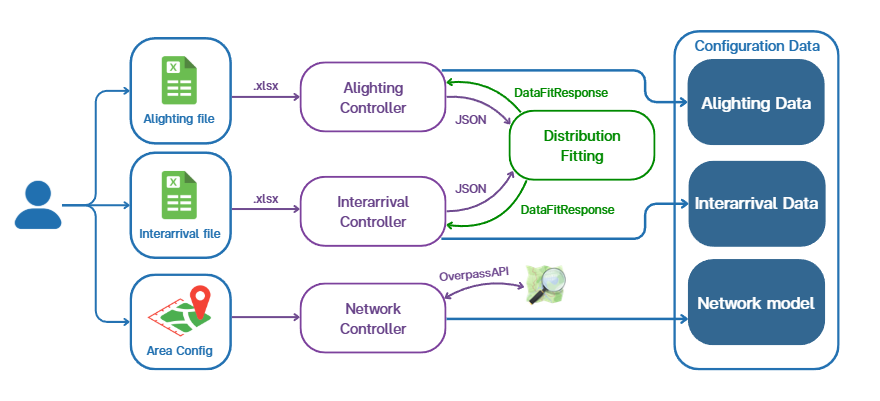
\includegraphics[width=\textwidth,height=0.9\textheight,keepaspectratio]{configuration_flow.png}
    \caption{การทำงานของข้อมูลการกำหนดค่าในระบบ }
    \label{fig:configuration_flow}
\end{figure}

\subsection{การทำงานของข้อมูลสถานการณ์จากผู้ใช้ (Scenario flow)}
\begin{mypara}
  \indent ข้อมูลสถานการณ์ (scenario data) ประกอบด้วย 3 ส่วนซึ่งเป็นข้อมูลที่ผู้ใช้สามารถปรับเปลี่ยนพารามิเตอร์ได้บ่อย ๆ เพื่อจำลองสถานการณ์ต่าง ๆ ดังนี้ 
\begin{itemize}
  \item เส้นทางการให้บริการของรถในแต่ละสายบริการ (Route) โดยจะเก็บเป็นลำดับของสถานีที่รถจะวิ่งผ่านในแต่ละสายบริการซึ่งจะอ้างอิง Network model ที่สร้างจากข้อมูลขอบเขตพื้นที่ที่จะทำการจำลอง (map area configuration) ในส่วนของข้อมูลการกำหนดค่า (configuration data)
  \item ตารางเวลาการออกรถ (bus schedule) ส่วนนี้จะนำเข้าข้อมูลในรูปแบบไฟล์สกุล .xlsx ซึ่งจะมีข้อมูลเวลาการออกรถของแต่ละสายบริการ โดยจะนำมาใช้ในการกำหนดเวลาที่รถจะออกจากสถานีต้นทางในแต่ละรอบการเดินรถ
  \item ข้อมูลของรถซึ่งมี ความจุผู้โดยสารระยะทางที่สามารถวิ่งได้สูงสุด ความเร็วในการวิ่ง (bus information) การกำหนดข้อมูลของรถแต่แยกตามสายบริการจะช่วยให้สามารถจำลองสถานการณ์ที่มีความหลากหลายของรถในแต่ละสายบริการได้อย่างเหมาะสม
\end{itemize}
โดยหลังจากข้อมูลแต่ละส่วนผ่านกระบวนการข้างต้นแล้ว ทั้งหมดจะถูกรวมกันเป็นข้อมูลสถานการณ์ (scenario data) นำไปรวมกับข้อมูลการกำหนดค่า (configuration data) ช่วงเวลาการจำลอง (time period) และ ช่วงเวลาย่อย (time slot) จากนั้นข้อมูลจะถูกประมวลผลผ่านแบบจำลอง ดังในภาพ \ref{fig:scenario_flow}
\end{mypara}

\begin{figure}[H]
    \centering
  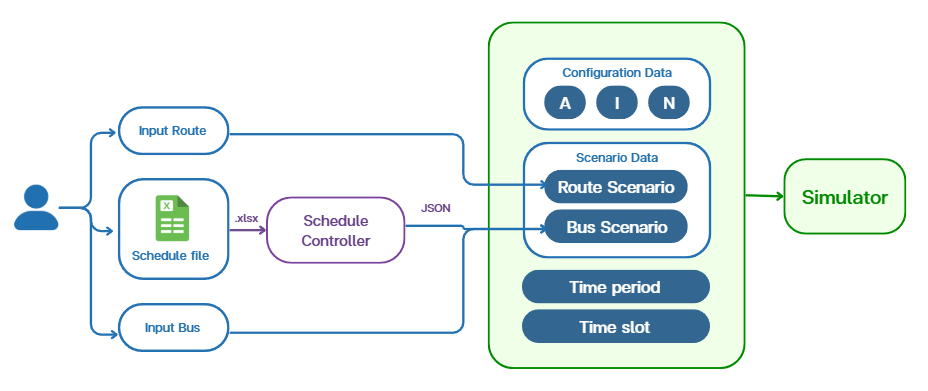
\includegraphics[width=\textwidth,height=0.9\textheight,keepaspectratio]{scenario_flow.png}
    \caption{การทำงานของข้อมูลสถานการณ์จากผู้ใช้ }
    \label{fig:scenario_flow}
\end{figure}

\subsection{ส่วนประมวลผลการจำลอง (Simulation engine)}
\begin{mypara}
  \indent ส่วนประมวลผลการจำลอง (simulation engine) มีส่วนประกอบหลักดังนี้
\begin{itemize}
  \item Helper functions ได้แก่ Mapper เป็นส่วนที่ทำหน้าที่เปลี่ยน JSON ให้เป็นตัวแปรที่ใช้คำนวณใน Python และ Timer เป็นตัวช่วยในเวลาในระบบจำลองมีค่าสอดคล้องกับเวลาการจำลองที่ผู้ใช้กำหนดไว้
  \item Simulator เป็นส่วนที่ทำหน้าที่ในการจำลองระบบขนส่งสาธารณะตามข้อมูลที่ได้รับจากส่วน scenario data และ configuration data ซึ่งจะใช้เทคนิคการจำลองแบบเหตุการณ์ไม่ต่อเนื่อง (discrete-event simulation) 
  และเทคนิคการจำลองแบบสุ่มเชิงสถิติ (stochastic simulation) ในการจำลองระบบขนส่งสาธารณะ ส่วนนี้จะมีองค์ประกอบย่อย 4 ส่วน ได้แก่ Bus Station Passenger และ Arrival Generator
  \item Output Generator เป็นส่วนที่ทำหน้าที่ในการสร้างผลลัพธ์เชิงสถิติที่สะท้อนประสิทธิภาพของระบบขนส่งสาธารณะมาแสดงผลในส่วน output โดยจะมีองค์ประกอบย่อย 2 ส่วน ได้แก่ Monitor และ Logger
\end{itemize}
  \indent ซึ่งแต่ละส่วนจะทำงานผสานในรูปแบบที่แสดงในภาพ \ref{fig:simulation_engine} และในส่วนนี้สัมพันธ์กับข้อมูลสถานการณ์ (scenario data) และข้อมูลการกำหนดค่า (configuration data) ดังในภาพ \ref{fig:simulation_overview} โดยข้อมูลสถานการณ์และข้อมูลการกำหนดค่าจะถูกนำไปใช้ในส่วนของ Simulator เพื่อจำลองระบบขนส่งสาธารณะ และผลลัพธ์ที่ได้จากการจำลองจะถูกส่งไปยัง Output Generator เพื่อสร้างผลลัพธ์เชิงสถิติที่สะท้อนประสิทธิภาพของระบบขนส่งสาธารณะมาแสดงผลในส่วน output
\end{mypara}

\begin{figure}[H]
    \centering
  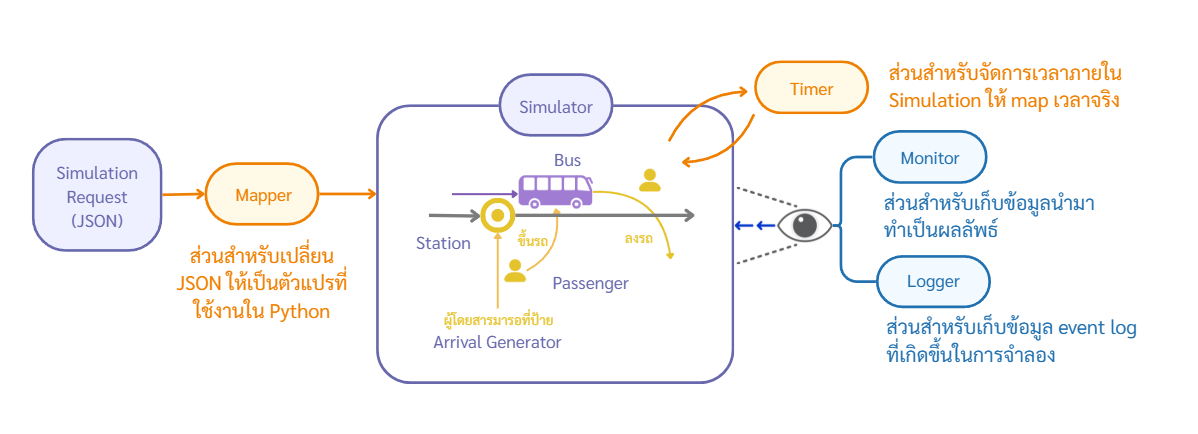
\includegraphics[width=\textwidth,height=0.9\textheight,keepaspectratio]{simulation_engine.png}
    \caption{การทำงานของส่วนประมวลผลการจำลอง }
    \label{fig:simulation_engine}
\end{figure}

\begin{figure}[H]
    \centering
  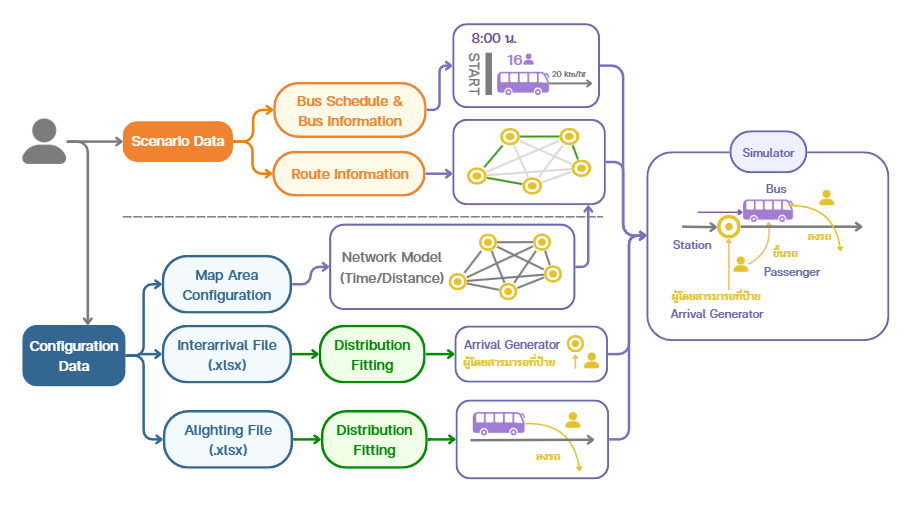
\includegraphics[width=\textwidth,height=0.9\textheight,keepaspectratio]{simulation_overview.png}
    \caption{ภาพรวมของการทำงานของส่วนประมวลผลการจำลอง }
    \label{fig:simulation_overview}
\end{figure}


\section{ส่วนติดต่อผู้ใช้ (User Interface)}
\begin{mypara}
    \indent โครงงานนี้มีการออกแบบเพื่อให้ผู้ใช้สามารถป้อนข้อมูลที่จำเป็นสำหรับ
    การจำลองระบบขนส่งสาธารณะได้อย่างสะดวกและไม่ซับซ้อน 
    โดยข้อมูลที่มีการเปลี่ยนแปลงบ่อย จะถูกจัดให้อยู่ในส่วนของ input 
    ซึ่งสามารถเข้าถึงและแก้ไขได้ง่ายโดยไม่ต้องผ่านขั้นตอนที่ซับซ้อน 
    ส่วนข้อมูลพื้นฐานของระบบขนส่งสาธารณะ จะถูกจัดเก็บแยกเป็น configuration data 
    เพื่อให้ง่ายต่อการนำมาใช้ซ้ำ และมี workspace สำหรับการจัดการข้อมูลที่ช่วยให้ผู้ใช้สามารถ 
    clone configuration data หรือ scenario data จากผู้อื่นมาใช้งานและปรับแก้ได้สะดวก

  \indent ในส่วนของ output ได้ออกแบบให้สามารถแสดงผลได้ทั้งมุมมองภาพรวมและ
  รายละเอียดรายสถานี เพื่อให้ผู้ใช้ตรวจสอบข้อมูลเชิงลึกได้อย่างครบถ้วน นอกจากนี้ยังมี 
  dashboard สรุปผล ที่นำเสนอข้อมูลในรูปแบบกราฟและตัวชี้วัดสำคัญ 
  เพื่อช่วยให้ผู้ใช้สามารถเปรียบเทียบและวิเคราะห์ประสิทธิภาพของระบบขนส่งสาธารณะ
  ได้อย่างสะดวกและมีประสิทธิภาพ
\end{mypara}

\subsection{การจัดกลุ่มผู้ใช้ (User Grouping)}
\begin{mypara}
\indent โครงงานนี้มีการจัดกลุ่มผู้ใช้เป็น 2 กลุ่มหลัก ได้แก่
\begin{itemize}
    \item ผู้ใช้ที่ลงทะเบียน (Registered Users): กลุ่มของผู้ใช้ที่ผ่านการยืนยันตัวตนด้วย google oauth 
    จะสามารถเข้าถึงฟังก์ชันการทำงานของระบบได้ครบถ้วน โดยระบบจะใช้ข้อมูลโปรไฟล์และรูปภาพจากบัญชี google ในการระบุตัวตน
    \item ผู้ใช้ที่ไม่ได้ลงทะเบียน (Guest Users): กลุ่มของผู้ใช้ทั่วไปที่ไม่ได้สร้างบัญชี 
    สามารถใช้ระบบจำลองได้แบบจำกัดฟังก์ชัน โดยทำการจำลองและดูผลลัพธ์ได้ชั่วคราว 
\end{itemize}
\end{mypara}
\section{ผังการทำงานของผู้ใช้ (User Flow)}
\begin{mypara}
    \indent โครงงานนี้มีการออกแบบผังการทำงานของผู้ใช้ สำหรับผู้ใช้ทั้ง 2 กลุ่ม เพื่อให้ผู้ใช้สามารถเข้าถึงฟังก์ชันต่าง ๆ ของระบบได้อย่างเหมาะสม 
    โดยมีการออกแบบดังนี้
\end{mypara}
  \subsection{ผู้ใช้ที่ไม่ได้ลงทะเบียน (Guest Users)}
  \begin{mypara}
    \indent ผังการทำงานของผู้ใช้ที่ไม่ได้ลงทะเบียน จะถูกจำกัดการเข้าถึงฟังก์ชันบางส่วนของระบบโดยมี
    การทำงานคือเมื่อผู้ใช้เข้ามาสู่หน้าแรก (Landing page) ซึ่งผู้ที่ไม่ได้ลงทะเบียนจะเข้าใช้
    ในโหมด Guest user โดยจะต้องกำหนดค่า (Configuration data) เมื่อกำหนดข้อมูลที่จะใช้ได้แล้ว
    จะสามารถ เข้าสู่หน้าสำหรับการใส่ ข้อมูลสถานการณ์ (Scenario data) เพื่อกรอกข้อมูลสถานการณ์และปรับแต่งข้อมูลได้ เมื่อกรอกข้อมูลเสร็จ
    แล้วจะสามารถกดปุ่มดำเนินการเพื่อเริ่มการใช้แบบจําลอง (Simulation) หลังจากการจำลองเสร็จสิ้น
    ผู้ใช้จะสามารถเลือกดูผลลัพธ์ได้โดยเลือกดูได้ทั้งแบบ Dashboard สรุปผลข้อมูล หรือ Interacting Visualize
    ซึ่งจะเป็นข้อมูลทางสถิติที่เป็นผลลัพธ์ภาพรวมหรือข้อมูลรายละเอียดรายสถานี ดังภาพ \ref{fig:UserFlowUnregistered}
  \end{mypara}

  \subsection{ผู้ใช้ที่ลงทะเบียน (Registered Users)}
  
  \begin{mypara}
    \indent ผังการทำงานของผู้ใช้ที่ลงทะเบียน จะสามารถเข้าถึงฟังก์ชันทั้งหมดของระบบ โดยมี
    การทำงานคือ เมื่อผู้ใช้เข้ามาสู่หน้าแรก (Landing page) โดยผู้ใช้จะใช้โหมดลงทะเบียน ผู้ใช้สามารถลงชื่อเข้าใช้ผ่านการยืนยันตัวตนด้วย google oauth 
    แล้วจะสามารถเข้าสู่ระบบ (Login) ได้ หลังจากเข้าสู่ระบบผู้ใช้จะเข้าสู่หน้า My Project ซึ่งเป็นการจัดการงานทั้งหมดของผู้ใช้
    โดยเริ่มจากการเลือกหรือสร้างชุดข้อมูลกำหนดค่า (Configuration Data) เพื่อใช้เป็นฐานอ้างอิงในการจำลองระบบขนส่งสาธารณะ 
    จากนั้นจึงเข้าสู่ขั้นตอนการกรอกข้อมูลสถานการณ์ (Scenario Data) และปรับแต่งข้อมูลสถานการณ์และปรับแต่งข้อมูลได้ เมื่อกรอกข้อมูลเสร็จ
    แล้วจะสามารถกดปุ่มดำเนินการเพื่อเริ่มการใช้แบบจําลอง (Simulation) หลังจากการจำลองเสร็จสิ้น
    ผู้ใช้จะสามารถเลือกดูผลลัพธ์ได้โดยเลือกดูได้ทั้งแบบ Dashboard สรุปผลข้อมูล หรือ Interacting Visualize
    ซึ่งจะเป็นข้อมูลทางสถิติที่เป็นผลลัพธ์ภาพรวมหรือข้อมูลรายละเอียดรายสถานี 
    ดังภาพ \ref{fig:UserFlowRegistered} 
  \end{mypara}

  \begin{figure}
    \centering
    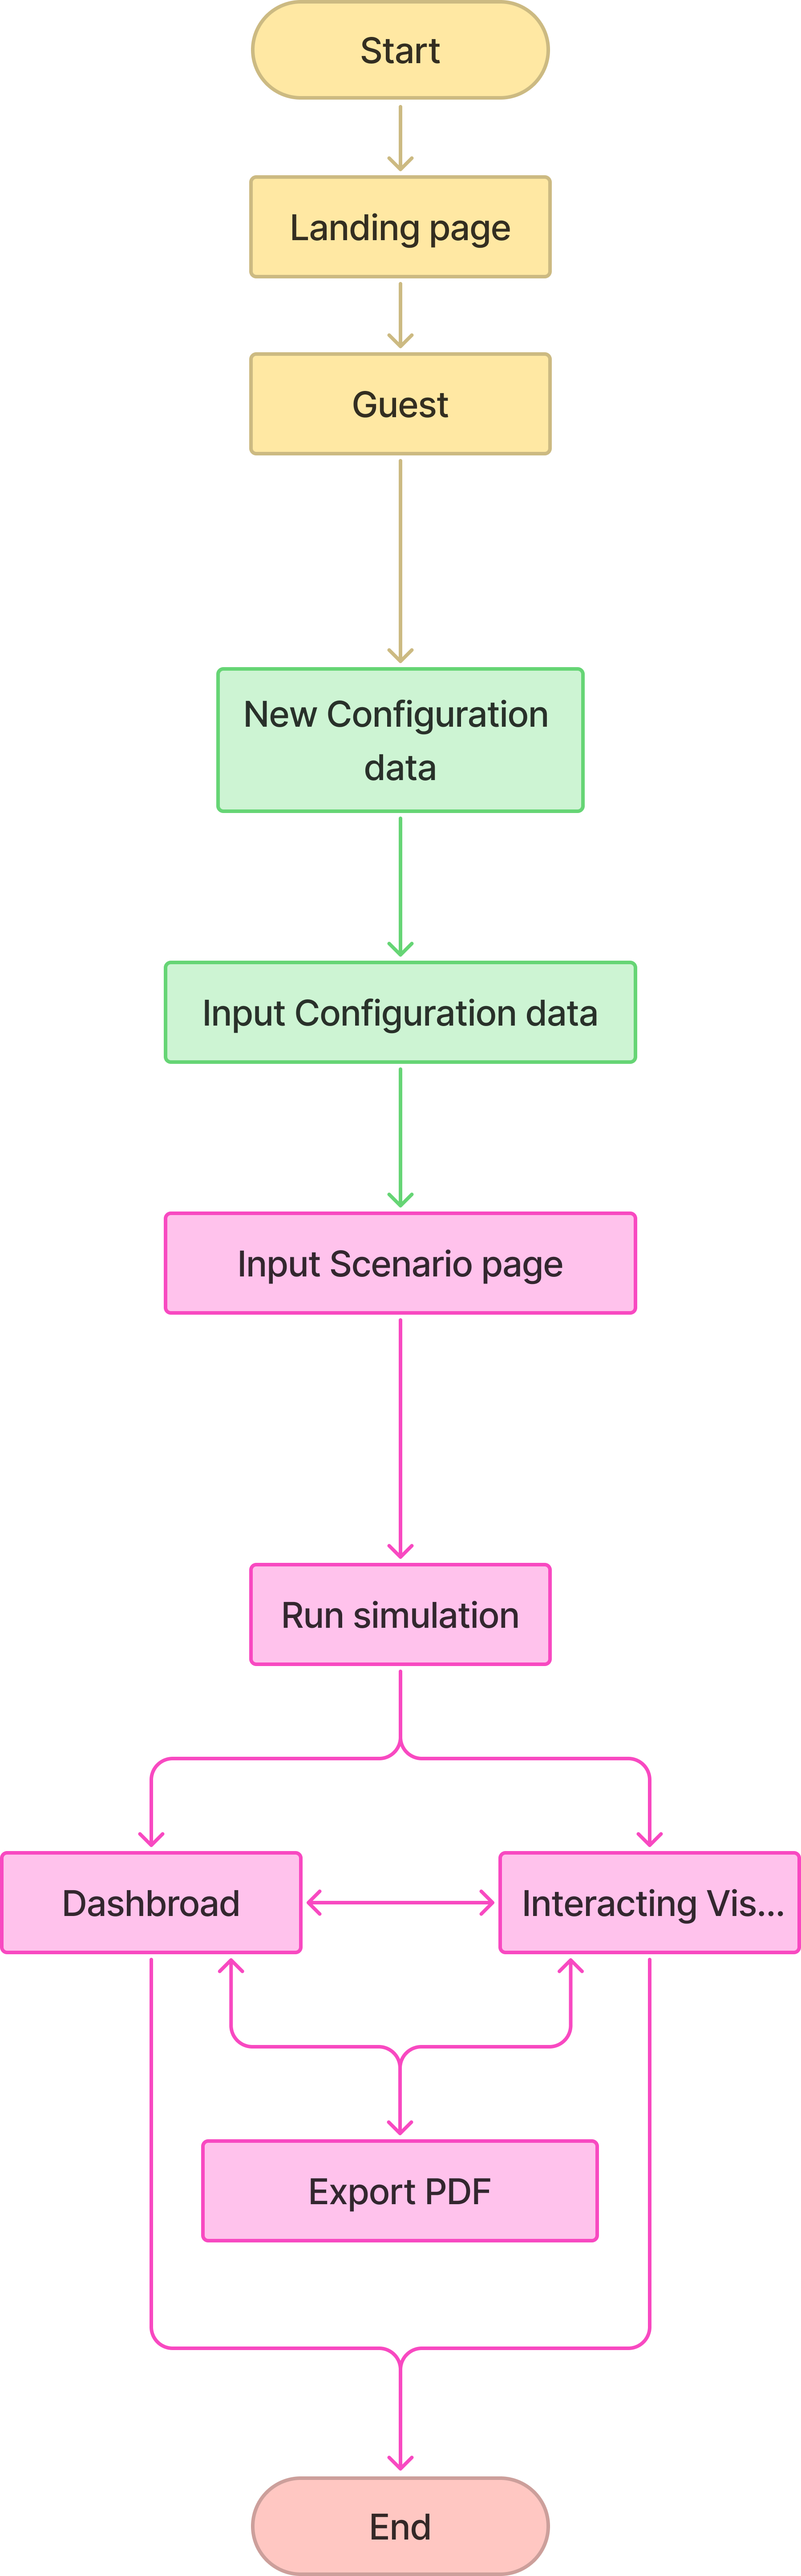
\includegraphics[width=\textwidth,height=0.95\textheight,keepaspectratio]{3-5Pic/UserFlowUnregistered.png}
    \caption{User flow  ของผู้ใช้ที่ไม่ได้ลงทะเบียน}
    \label{fig:UserFlowUnregistered}
  \end{figure}

    \begin{figure}
      \centering
      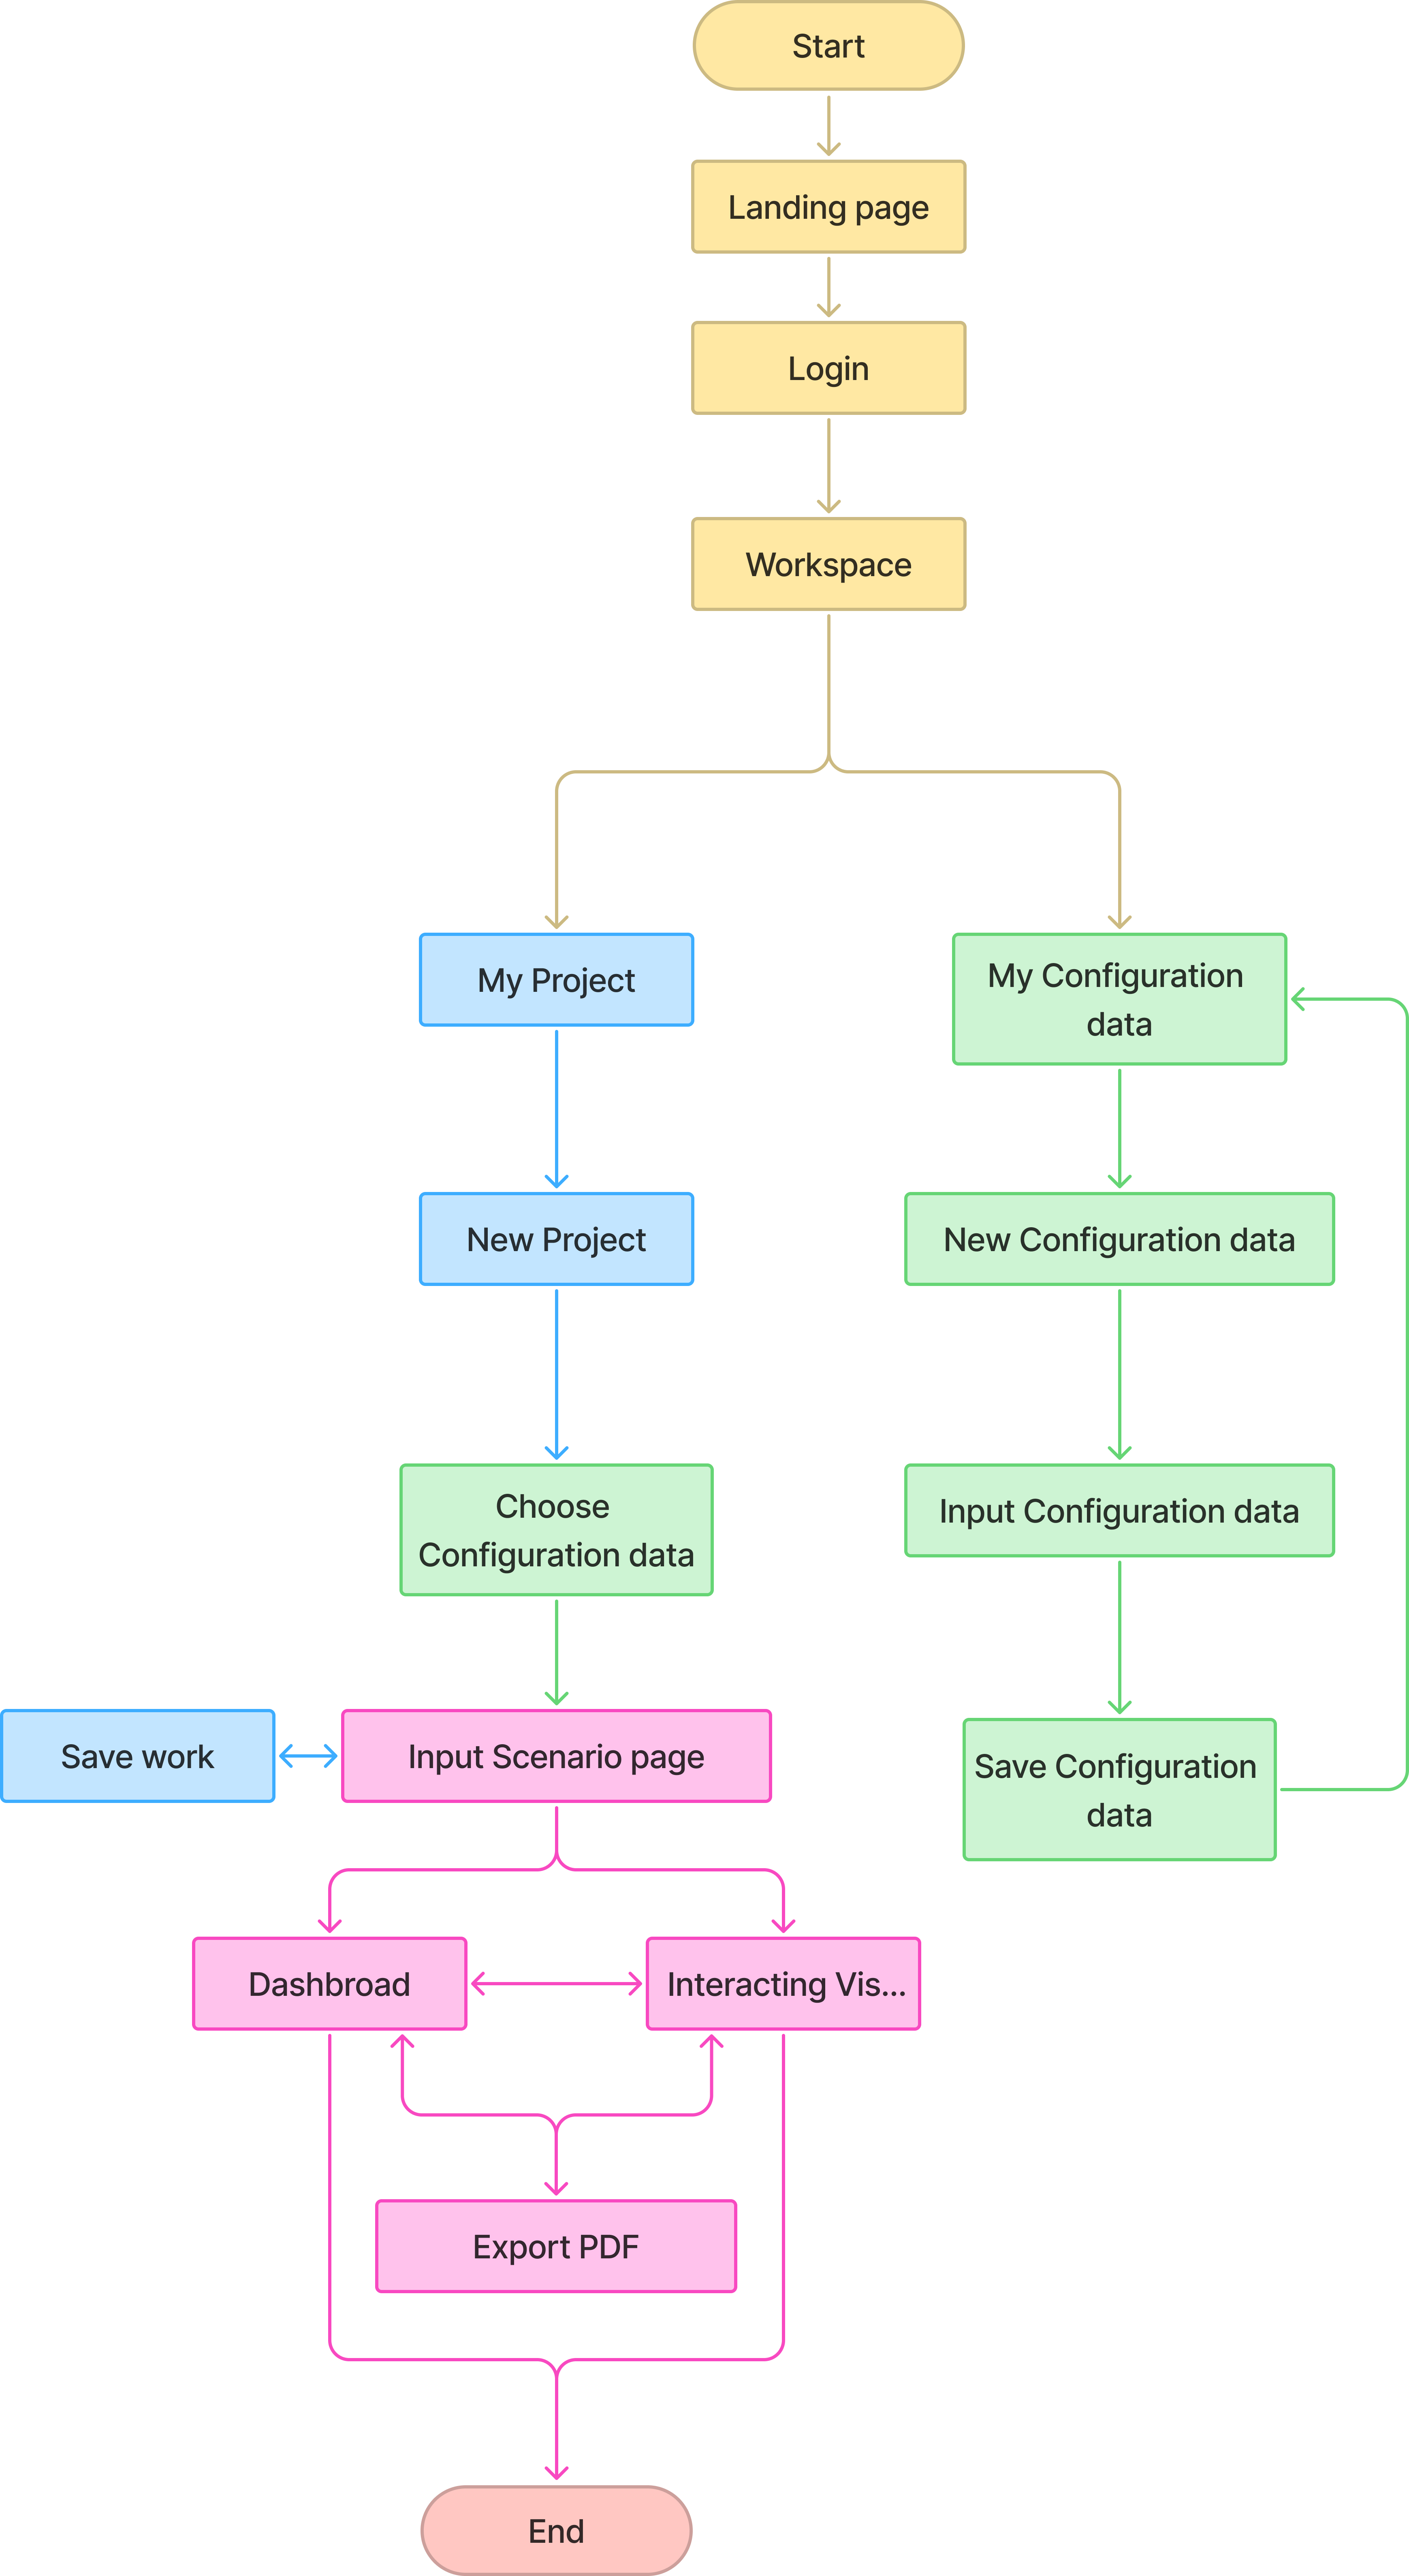
\includegraphics[width=\textwidth,height=0.95\textheight,keepaspectratio]{3-5Pic/UserFlowRegistered.png}
      \caption{User flow ของผู้ใช้ที่ลงทะเบียน}
      \label{fig:UserFlowRegistered}
    \end{figure}
      
\newpage
\section{การแสดงผลหน้าจอระบบ (System Interface)}
\begin{mypara}
    \indent โครงงานนี้ได้พัฒนาส่วนติดต่อผู้ใช้งาน (User Interface) ของระบบในหน้าต่างๆ 
    เพื่อรองรับการใช้งานจริง โดยมีรายละเอียดการทำงานของแต่ละหน้าจอดังนี้

\subsection{หน้าจอของผู้ใช้ที่ไม่ได้ลงทะเบียน (Guest Users / Unregistered Users)}
\begin{itemize}
    \item Step 1: ผู้ใช้จะเข้าสู่หน้า Landing page เพื่อเลือกระหว่างจะเข้าใช้ในโหมด Guest user หรือ Login user 
    ตามภาพ \ref{fig:Landpage}
      \begin{figure}[H]
        \centering
        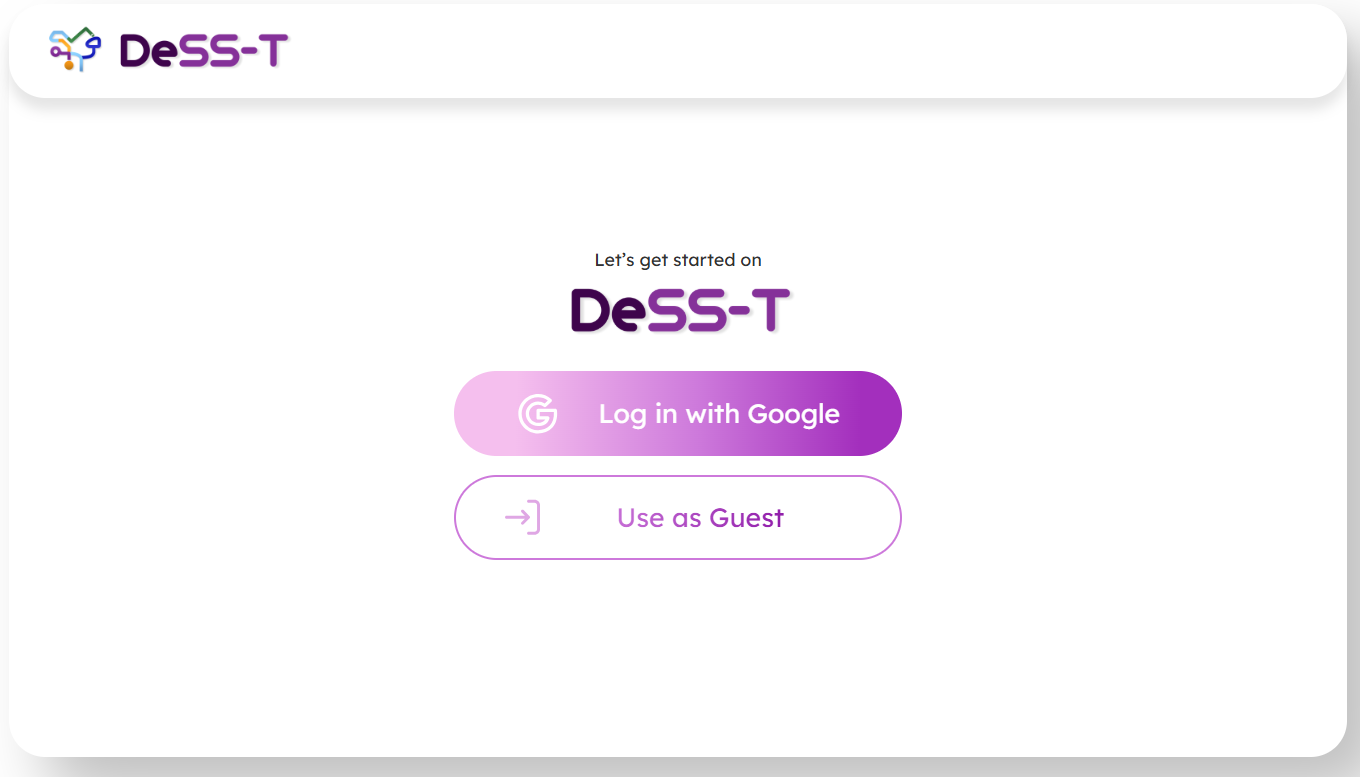
\includegraphics[scale=0.35]
        {3-5Pic/homepage_guest.png}
        \caption{หน้า Landing page}
        \label{fig:Landpage}
      \end{figure}
    
    \item Step 2: หากเลือก Guest user จะต้อง Setup ข้อมูลทั้งหมดเอง
    ตามภาพ \ref{fig:SetupConfigMapGuest} และ \ref{fig:SetupConfigDataGuest}
      \begin{figure}[H]
        \centering
        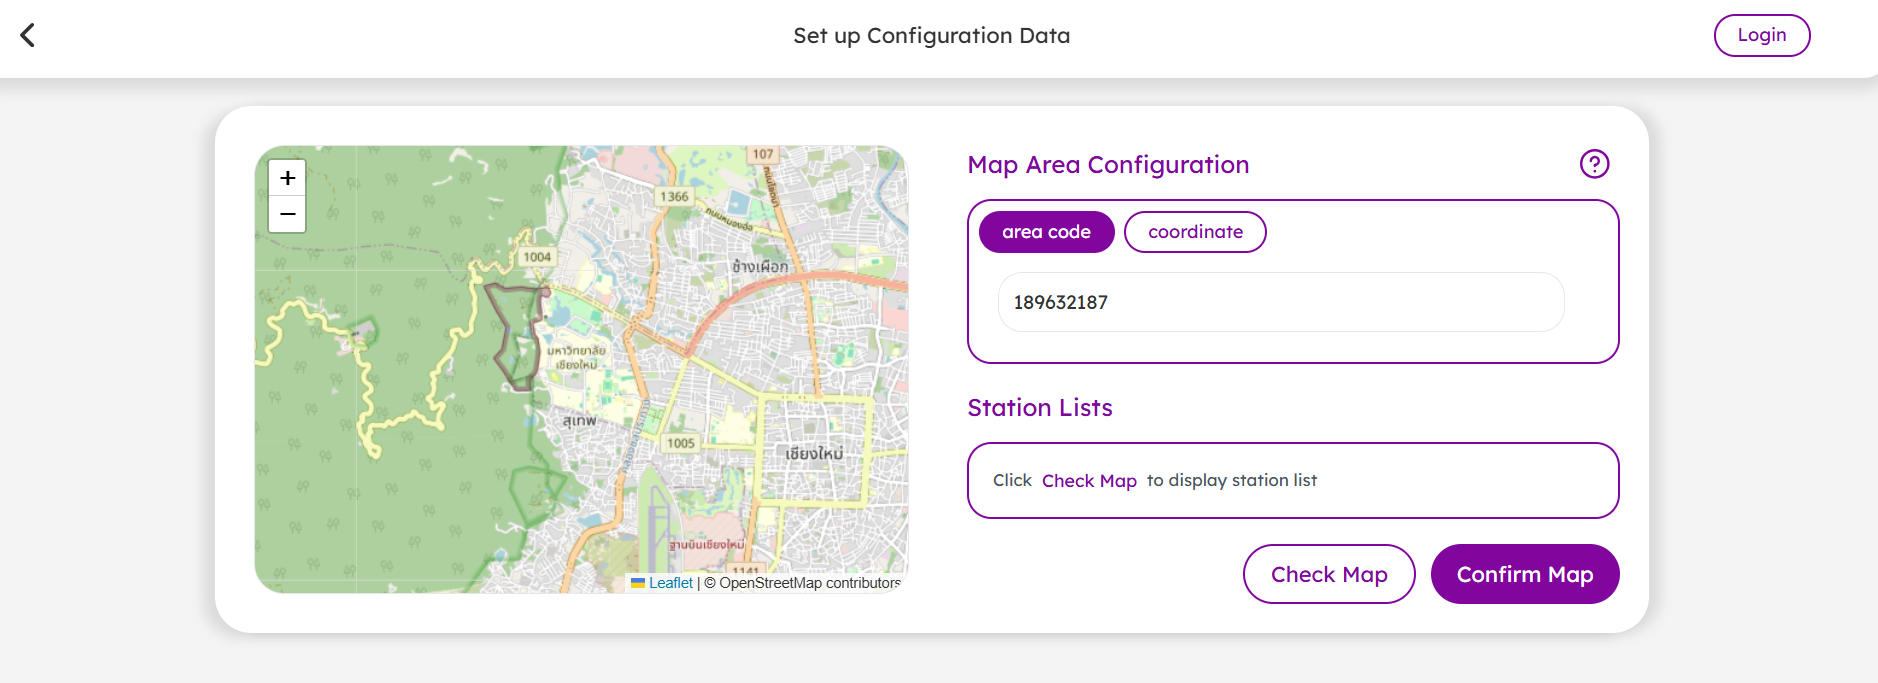
\includegraphics[scale=0.3]
        {3-5Pic/SetupConfigGuest.png}
        \caption{หน้า Setup Map area สำหรับ Guest}
        \label{fig:SetupConfigMapGuest}
      \end{figure}
      \begin{figure}[H]
        \centering
        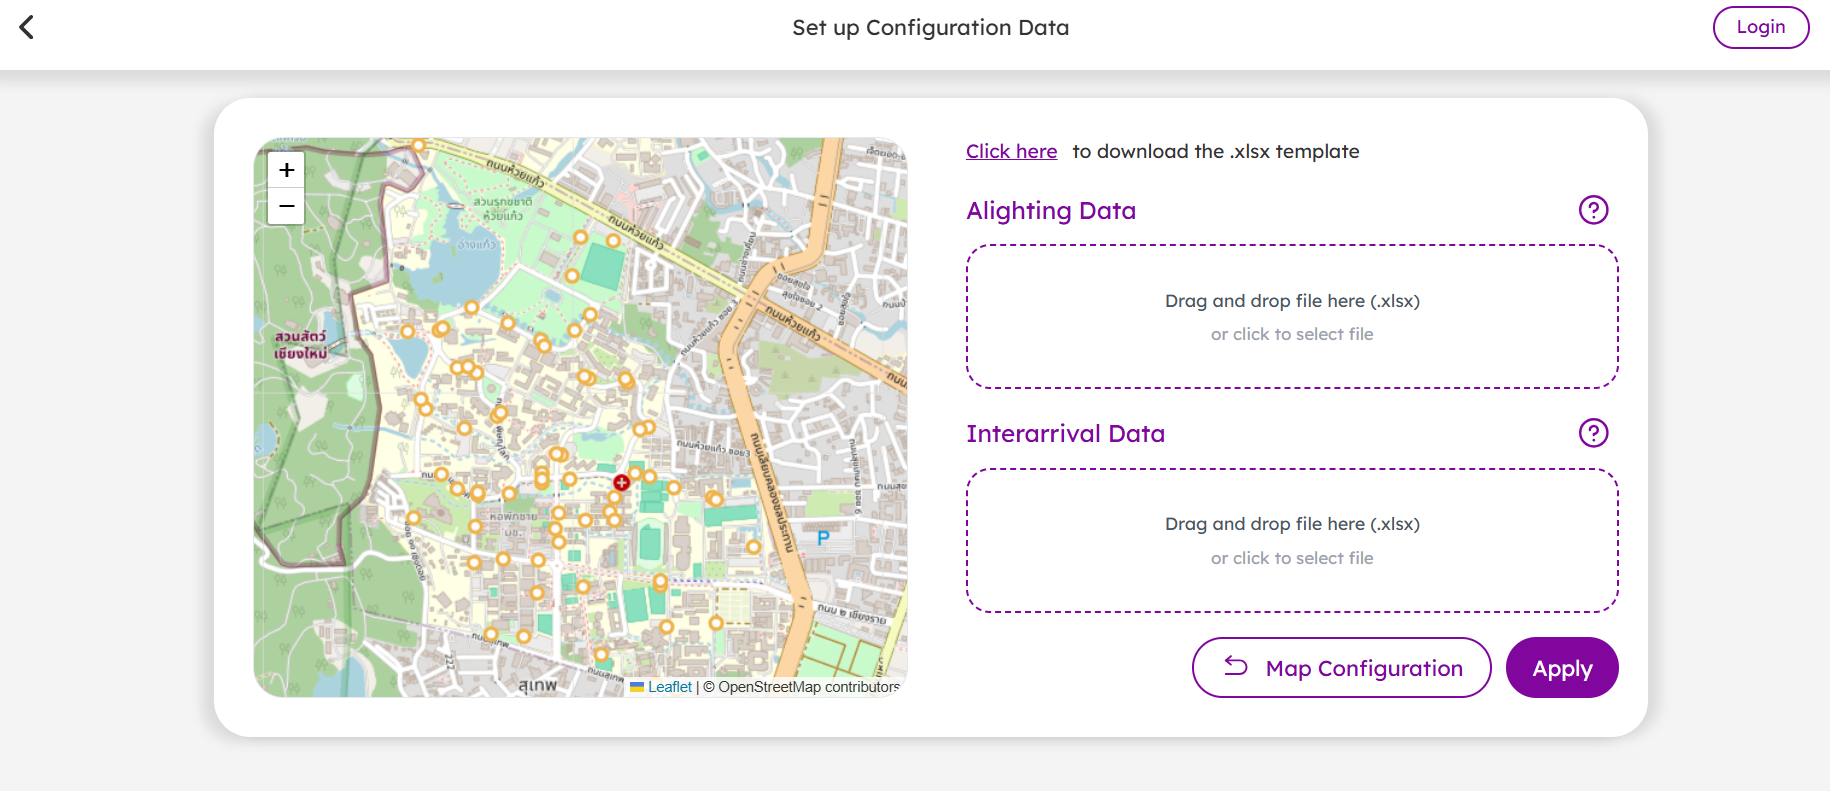
\includegraphics[scale=0.3]
        {3-5Pic/SetupConfigDataGuest.png}
        \caption{หน้า Setup Configuration data สำหรับ Guest}
        \label{fig:SetupConfigDataGuest}
      \end{figure}

    \item Step 3: หลังจาก Setup Configuration data ทั้งหมดเรียบร้อยจะเข้าสู่หน้า Input Scenario page 
    เพื่อกรอกข้อมูลสำหรับการจำลองบน Scenario ต่างๆ ตามภาพ \ref{fig:WireframeInputGuest} และ \ref{fig:WireframeInputRouteGuest}
      \begin{figure}[H]
        \centering
        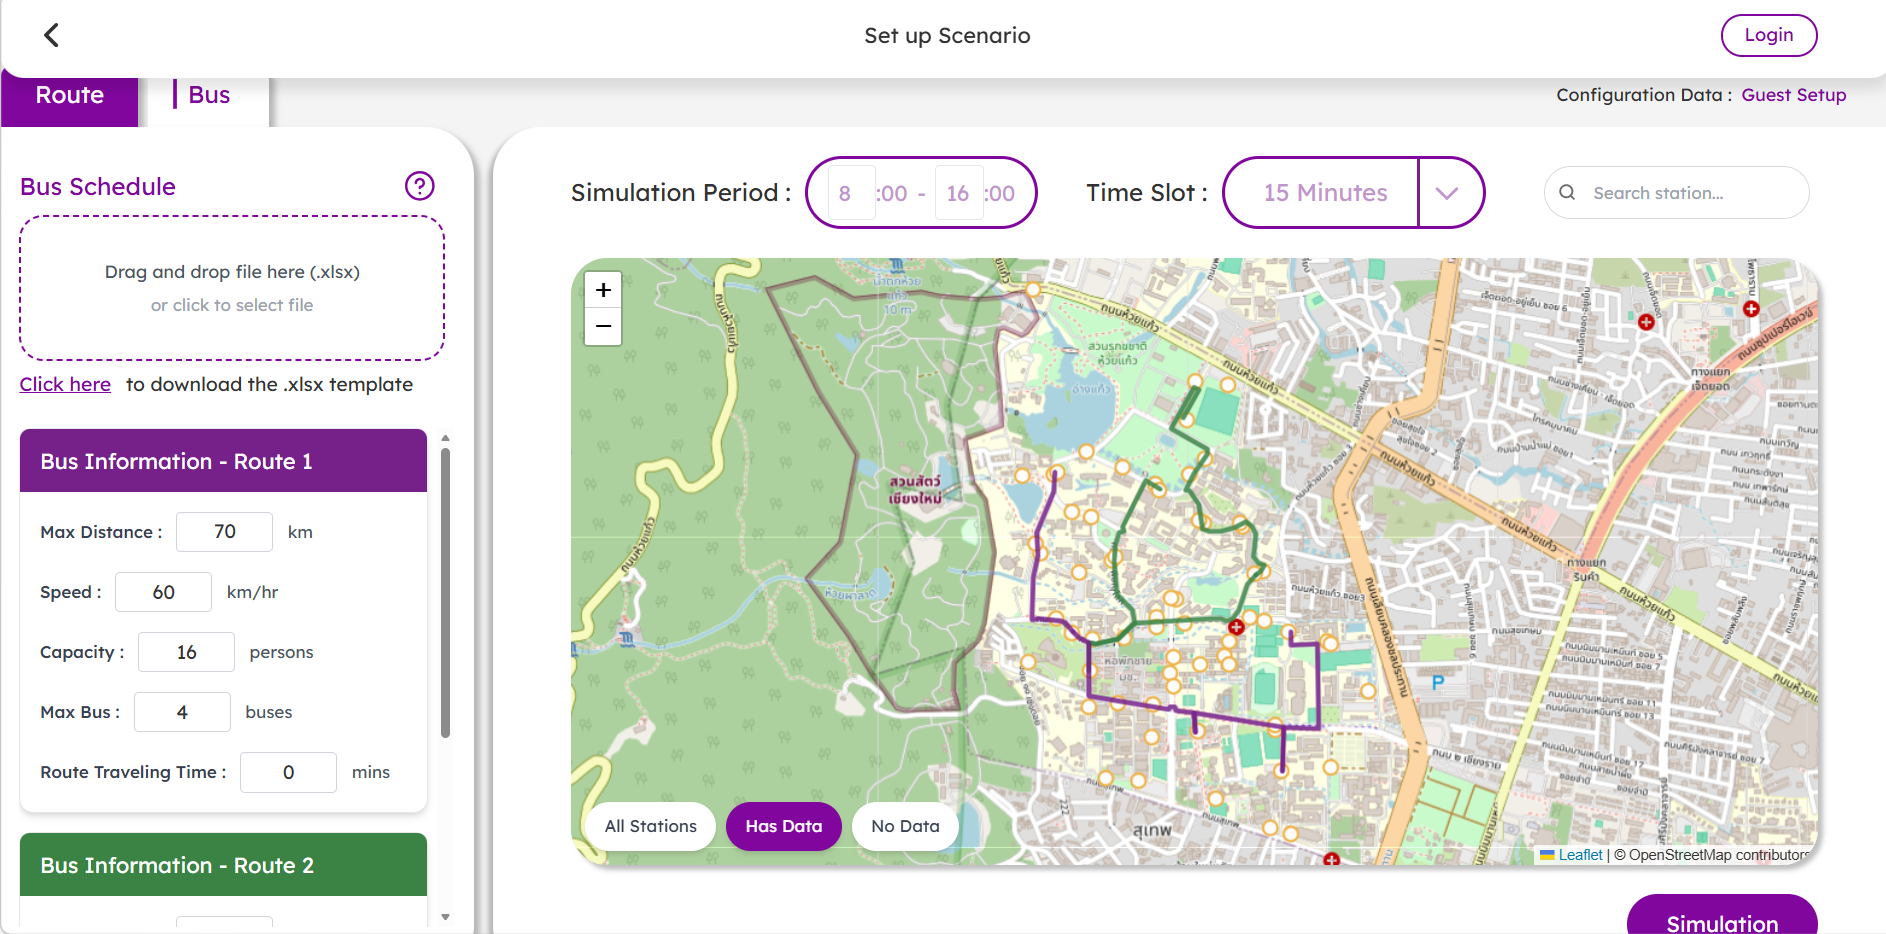
\includegraphics[scale=0.275]{3-5Pic/ScenarioBusGuest.png}
        \caption{หน้า Input Scenario page (bus) }
        \label{fig:WireframeInputGuest}
      \end{figure}
      \begin{figure}[H]
        \centering
        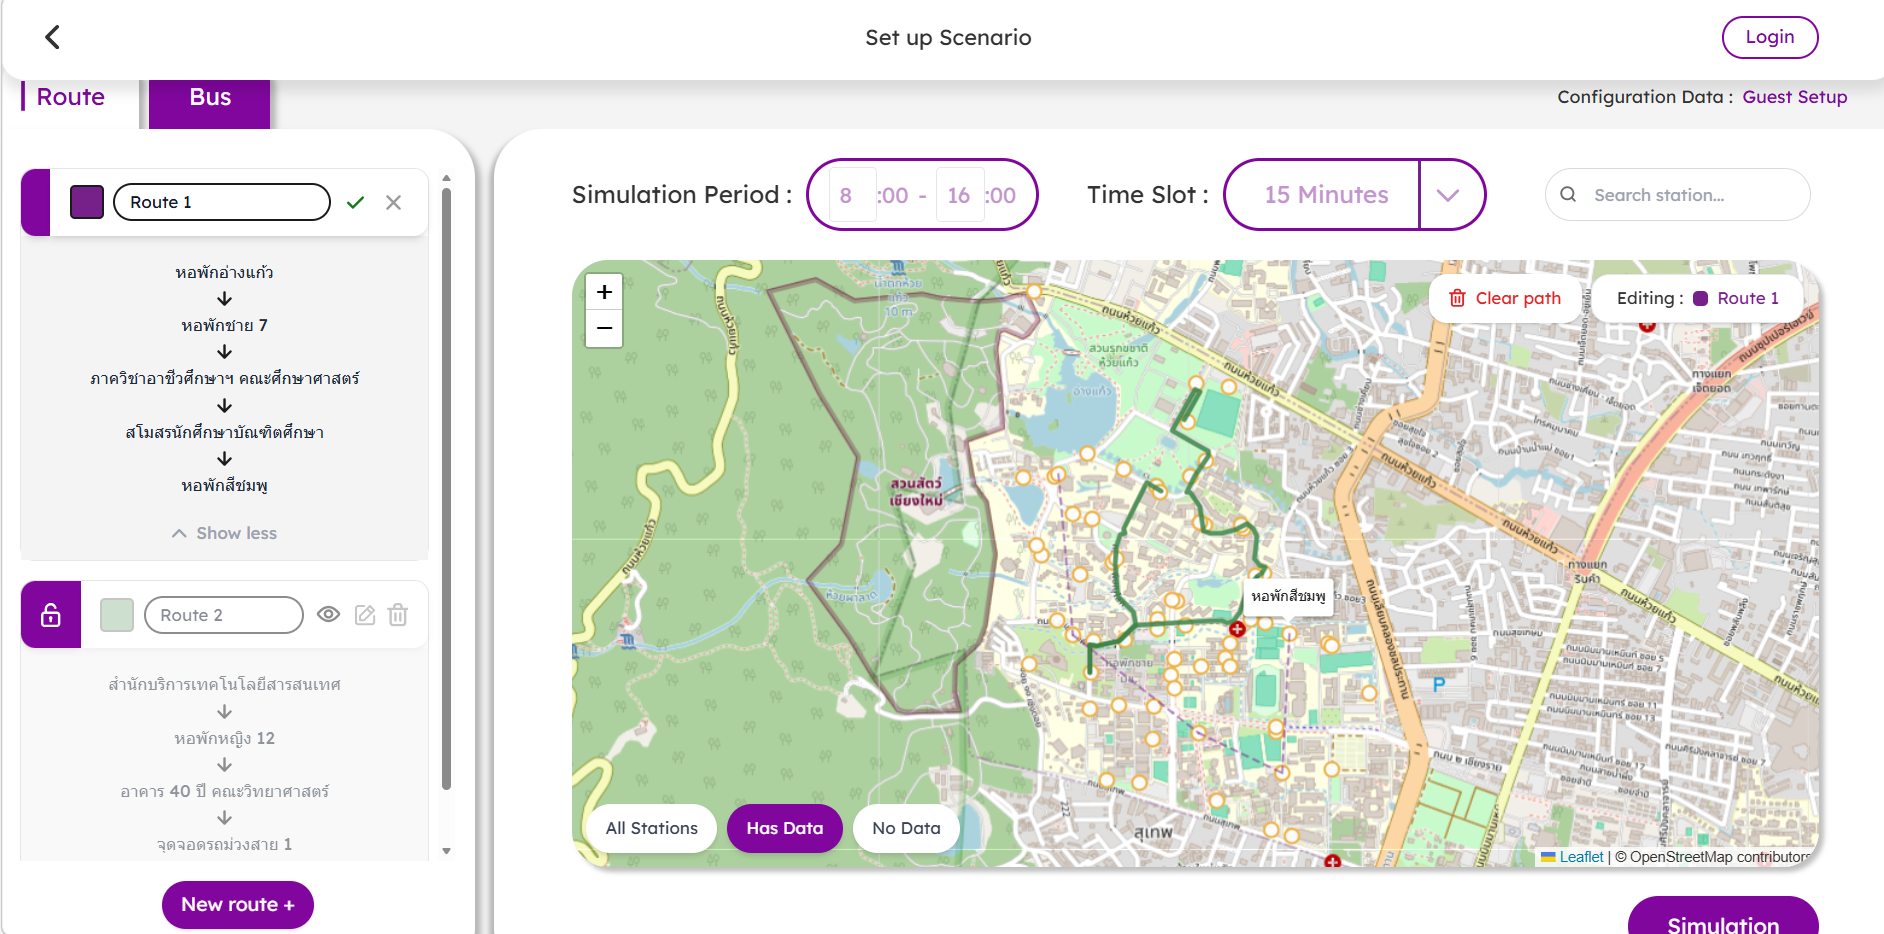
\includegraphics[scale=0.275]{3-5Pic/ScenarioRouteGuest.png}
        \caption{หน้า Input Scenario page (route) }
        \label{fig:WireframeInputRouteGuest}
      \end{figure}

    \item Step 4: หลังจากผู้ใช้กดปุ่ม Run simulation แล้ว User จะสามารถเลือกดู Dashboard สรุปผลข้อมูล 
    หรือ Interacting Visualize ตามภาพ \ref{fig:WireframeOutputGuest} และ \ref{fig:WireframeDashboardGuest}
      \begin{figure}[H]
        \centering
        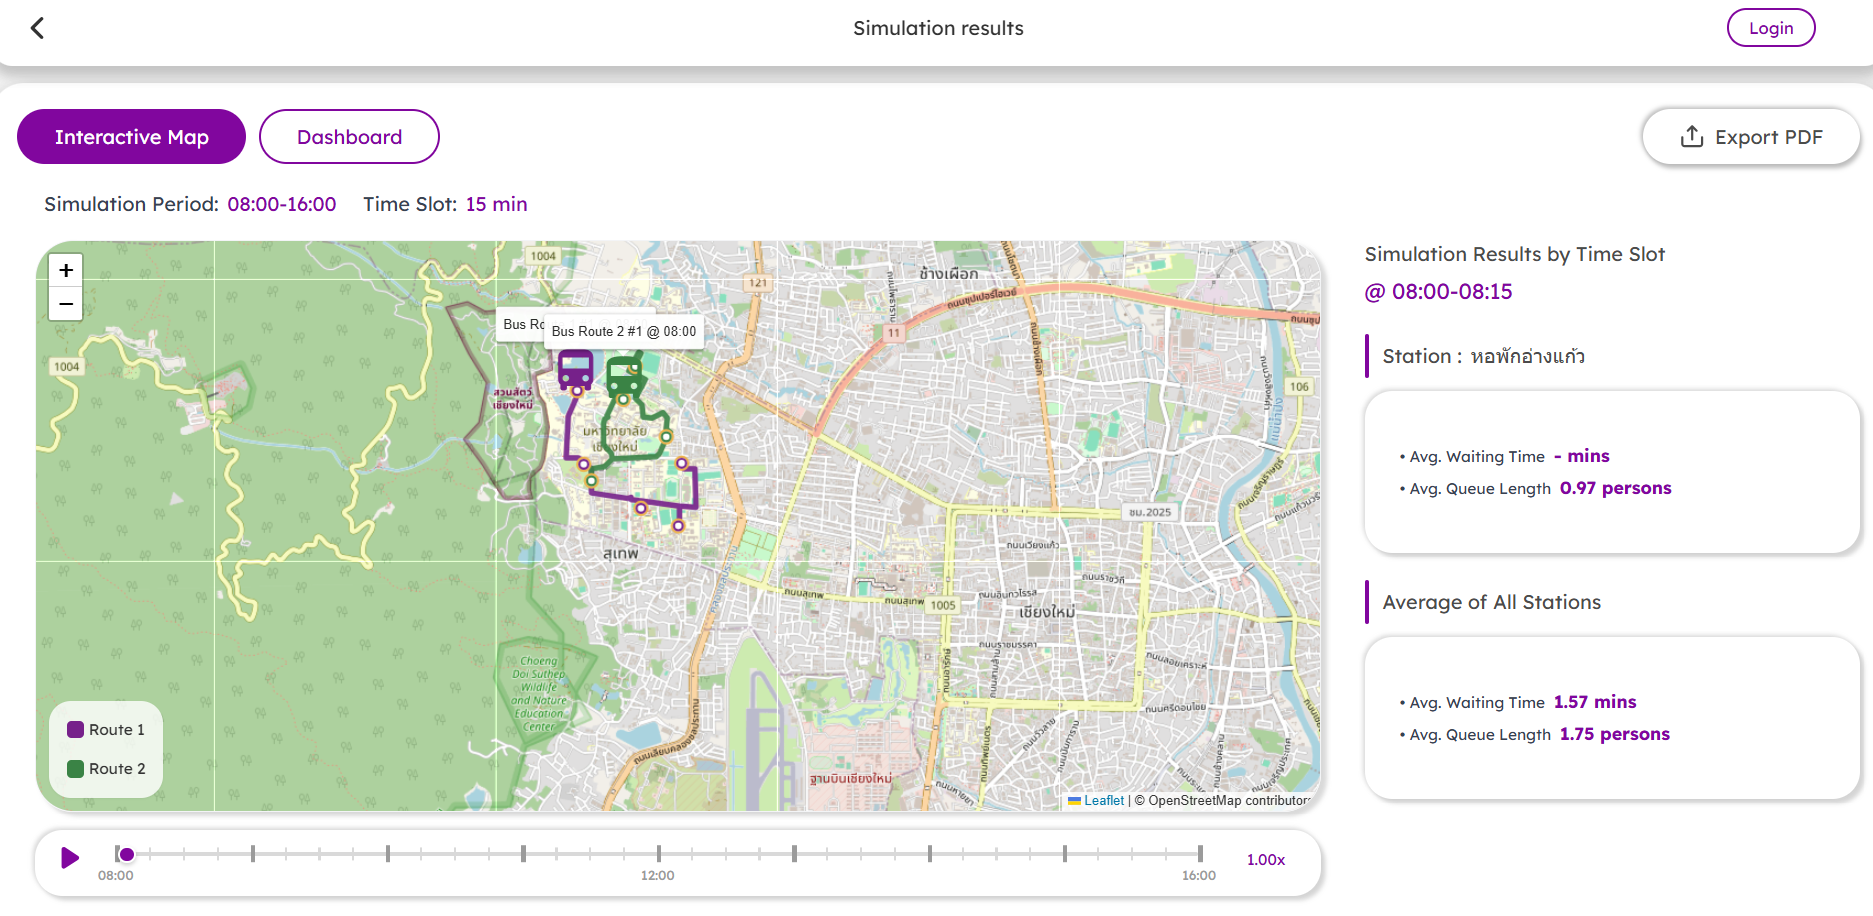
\includegraphics[scale=0.3]{3-5Pic/Interactive_MapGuest.png}
        \caption{หน้าแสดงผลลัพธ์หลังจาก Run Simulation}
        \label{fig:WireframeOutputGuest}
      \end{figure} 

      \begin{figure}[H]
        \centering
        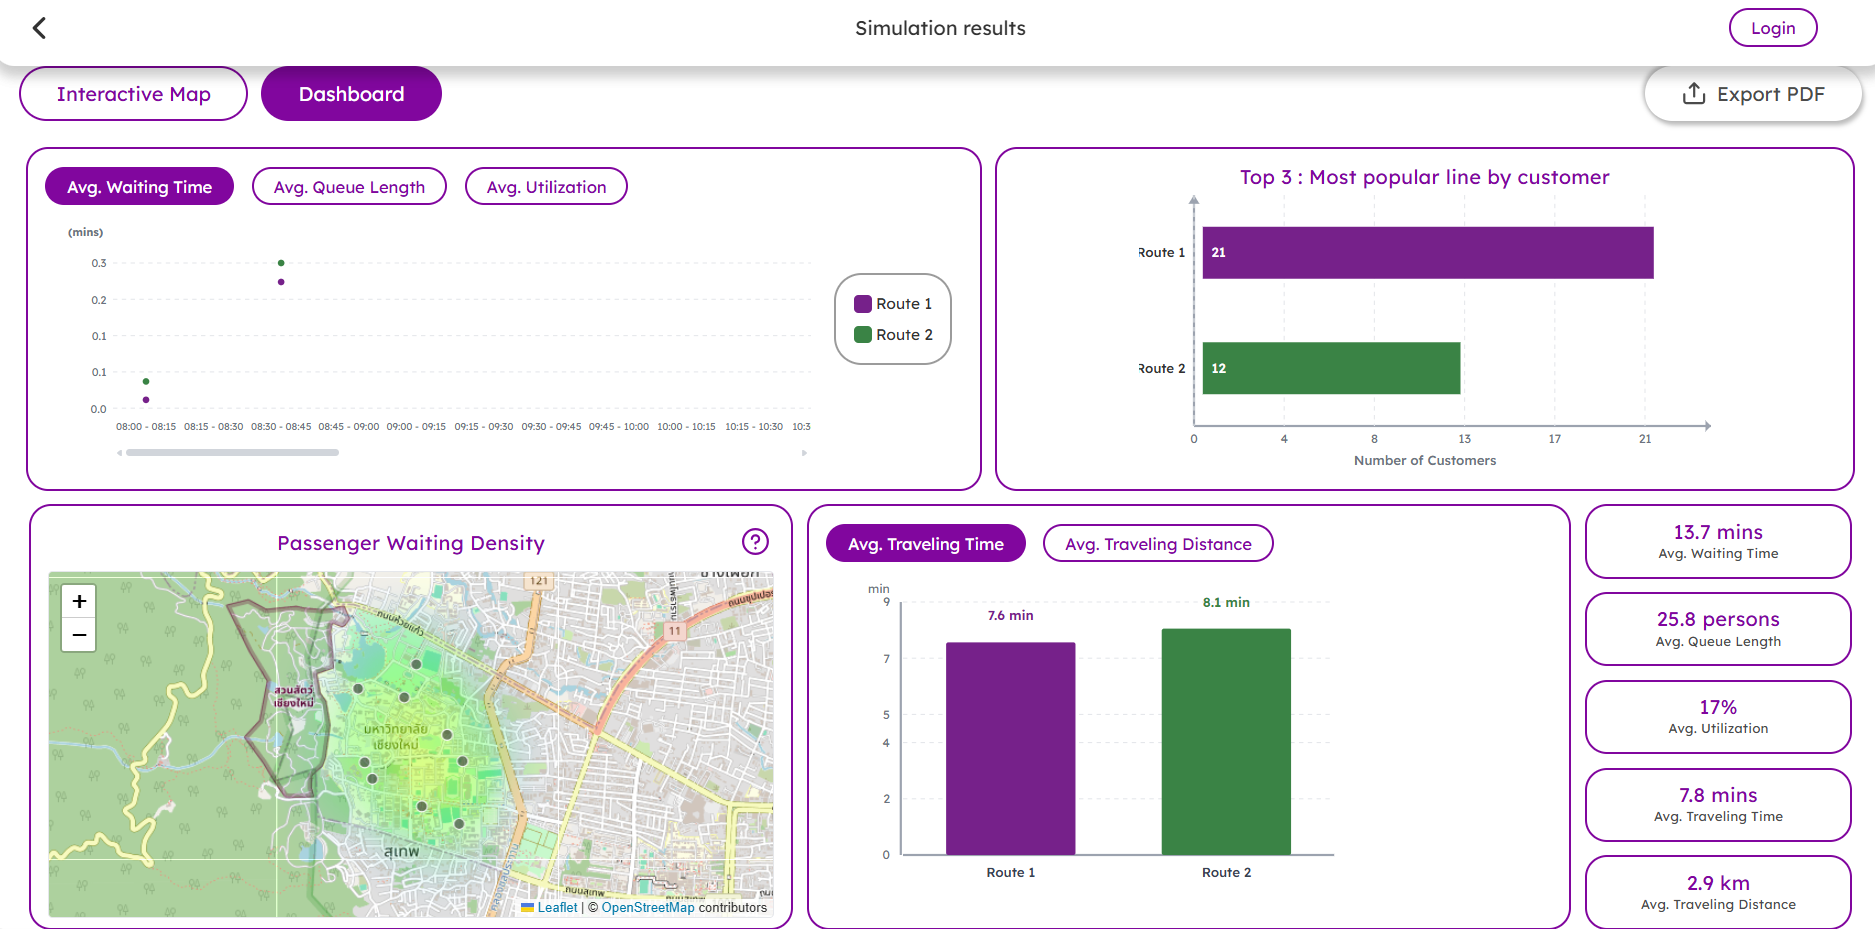
\includegraphics[scale=0.3]{3-5Pic/Dashboard_Guest.png}
        \caption{หน้า Dashboard }
        \label{fig:WireframeDashboardGuest}
      \end{figure}
    
      \item Step 5: ผู้ใช้สามารถกด Export PDF เพื่อดูและบันทึกข้อมูลที่จำลองออกมาแบบละเอียดได้ 
      ตามภาพ \ref{fig:ExportPDFGuest}
      \begin{figure}[H]
        \centering
        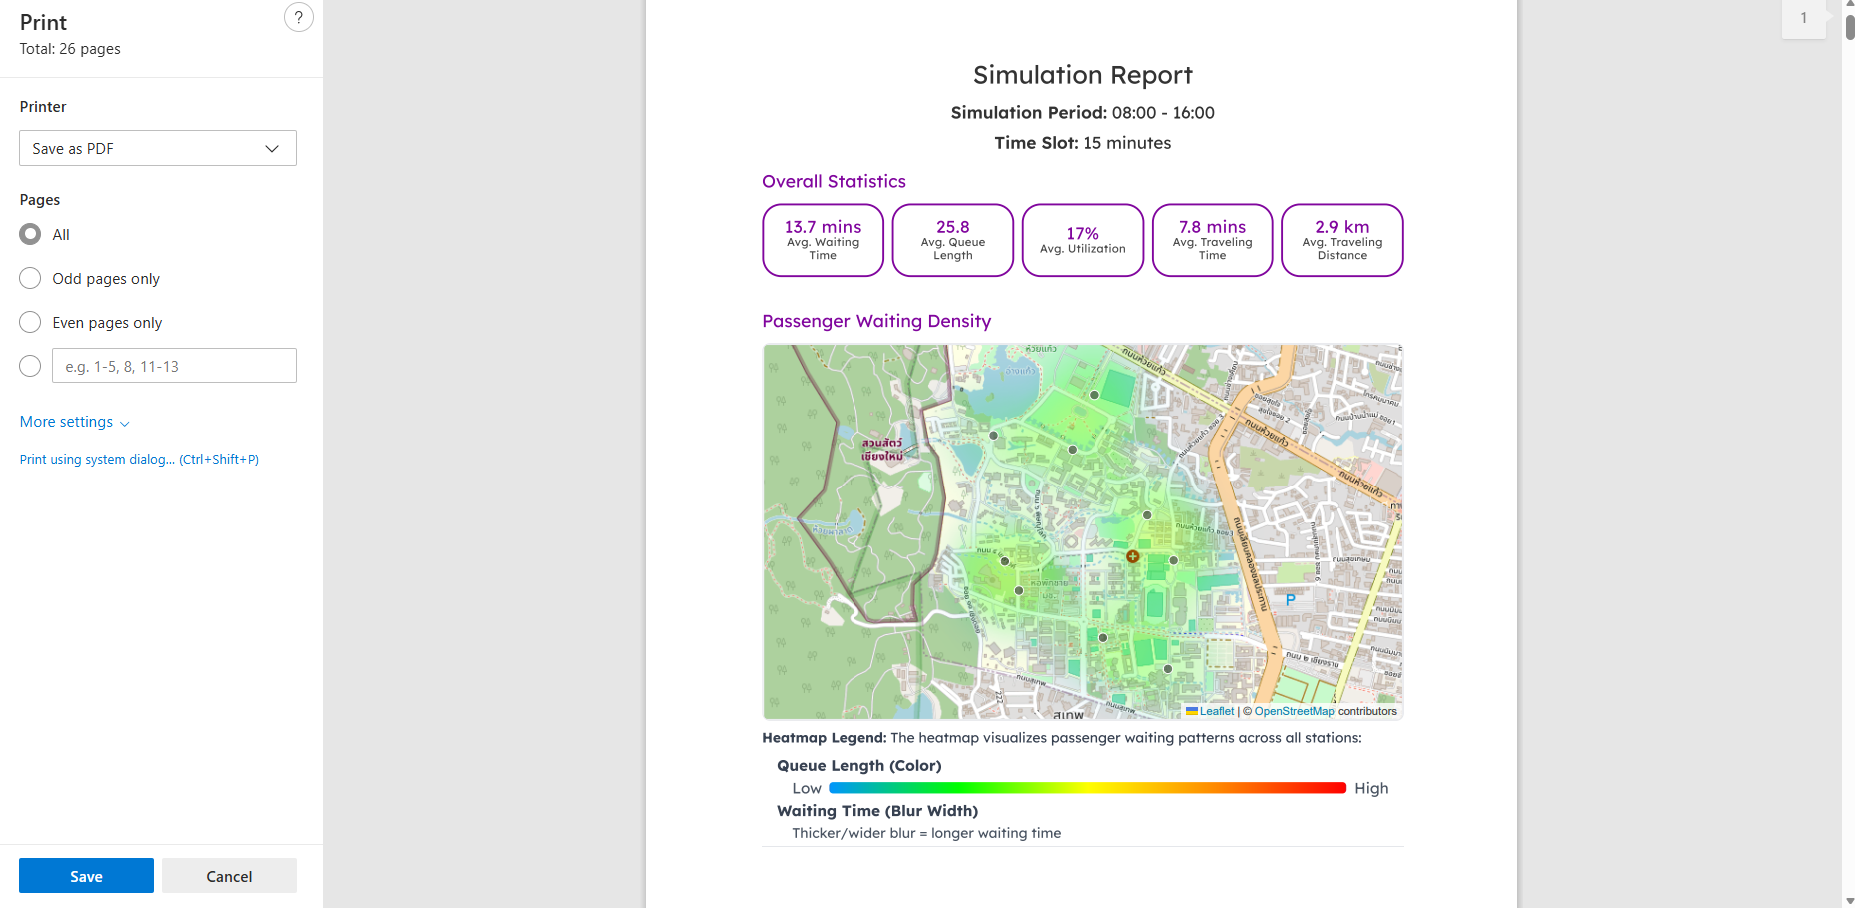
\includegraphics[scale=0.275]{3-5Pic/pdfGuest.png}
        \caption{หน้า Export PDF}
        \label{fig:ExportPDFGuest}
      \end{figure}

\end{itemize} 


\subsection{หน้าจอของผู้ใช้ที่ลงทะเบียน (Registered Users)}
\begin{itemize}
    \item Step 1:  ผู้ใช้จะเข้าสู่หน้า Landing page เพื่อเลือกระหว่างจะเข้าใช้ในโหมด Guest user หรือ Login user
    ตามภาพ \ref{fig:WireframeHomepageLogin}
    \begin{figure}[H]
    \centering
    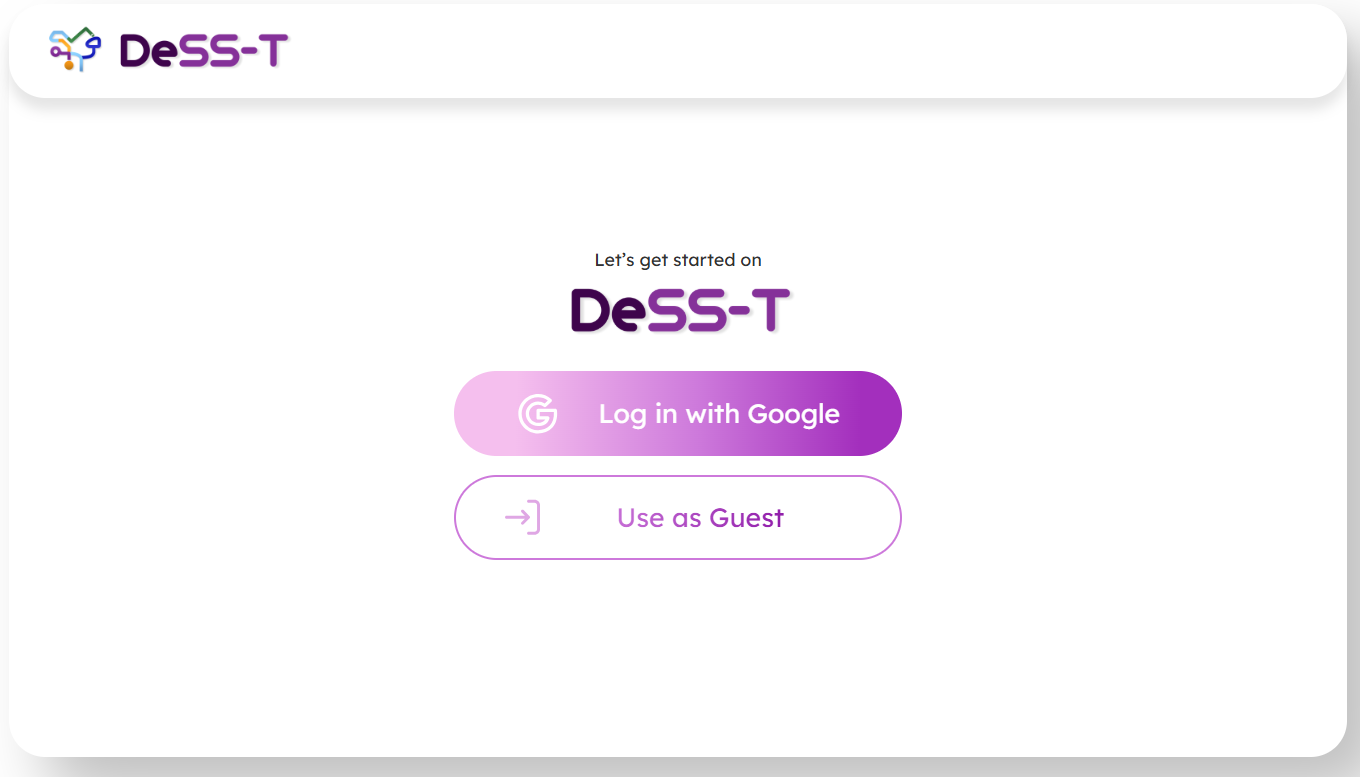
\includegraphics[scale=0.4]
    {3-5Pic/homepage_guest.png}
    \caption{หน้า Landing page}
    \label{fig:WireframeHomepageLogin}
    \end{figure}

    \item Step 2: หลังจากเข้าสู่ระบบผู้ใช้จะเข้าสู่หน้า My Project ซึ่งเป็นการจัดการงานทั้งหมดของผู้ใช้
    ตามภาพ \ref{fig:WireframeMyWork}
      \begin{figure}[H]
        \centering
        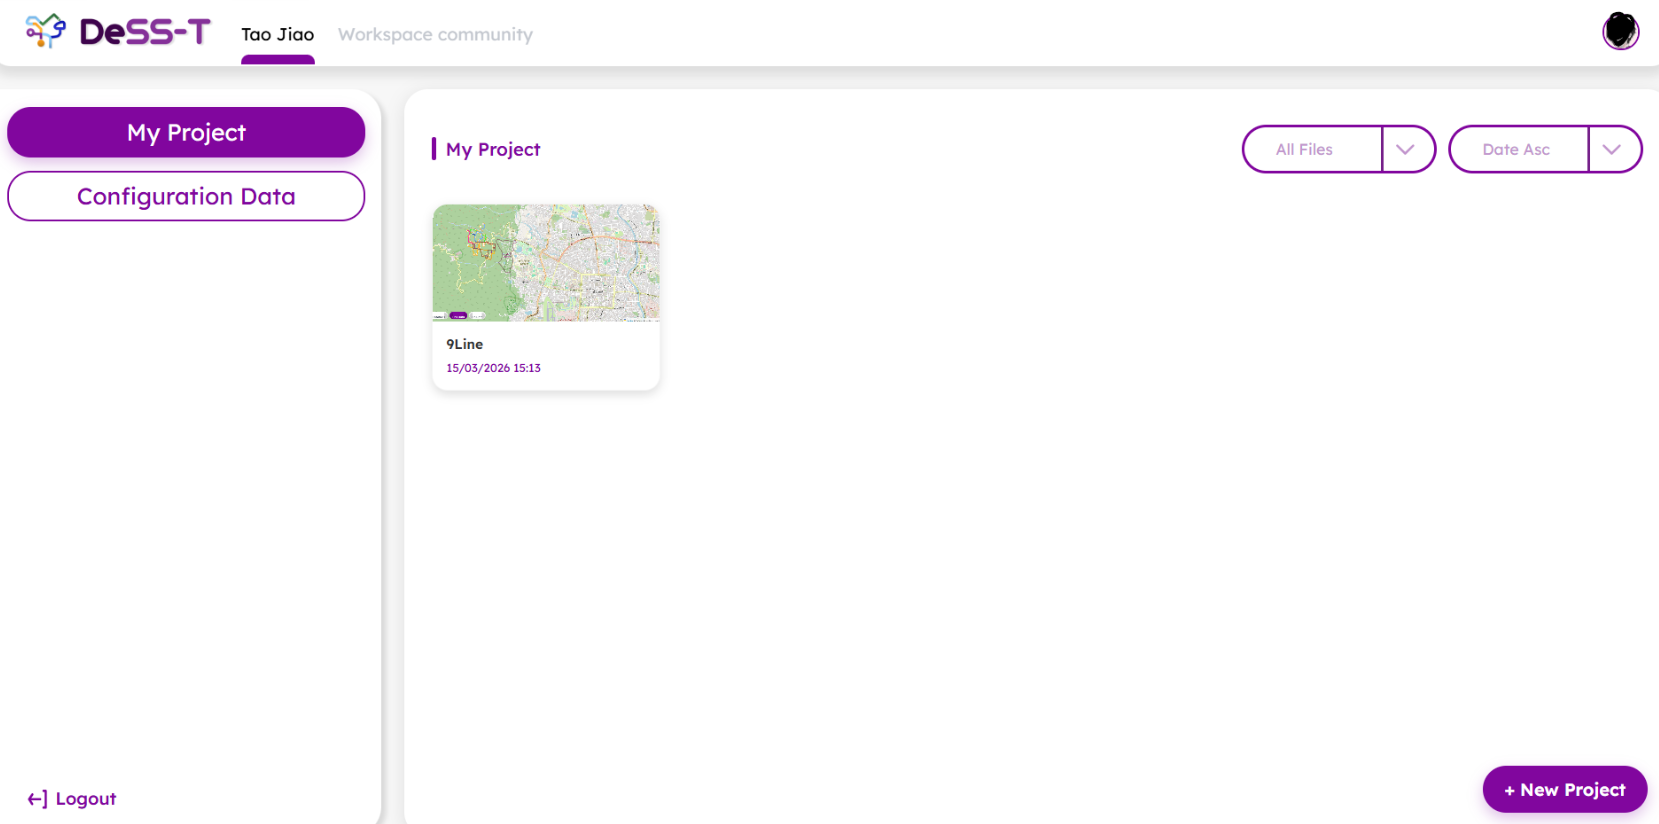
\includegraphics[scale=0.3]
        {3-5Pic/MyProject.png} 
        \caption{หน้า My Project}
        \label{fig:WireframeMyWork}
      \end{figure}
        
      \item  ผู้ใช้สามารถสร้าง Project ใหม่ได้ด้วยการกดที่ปุ่ม New Project โดยการสร้าง Project จะต้องอ้างอิงกับ Configuration data ที่มีอยู่
      ตามภาพ \ref{fig:WireframeNewWork}  
      \begin{figure}[H]
        \centering
        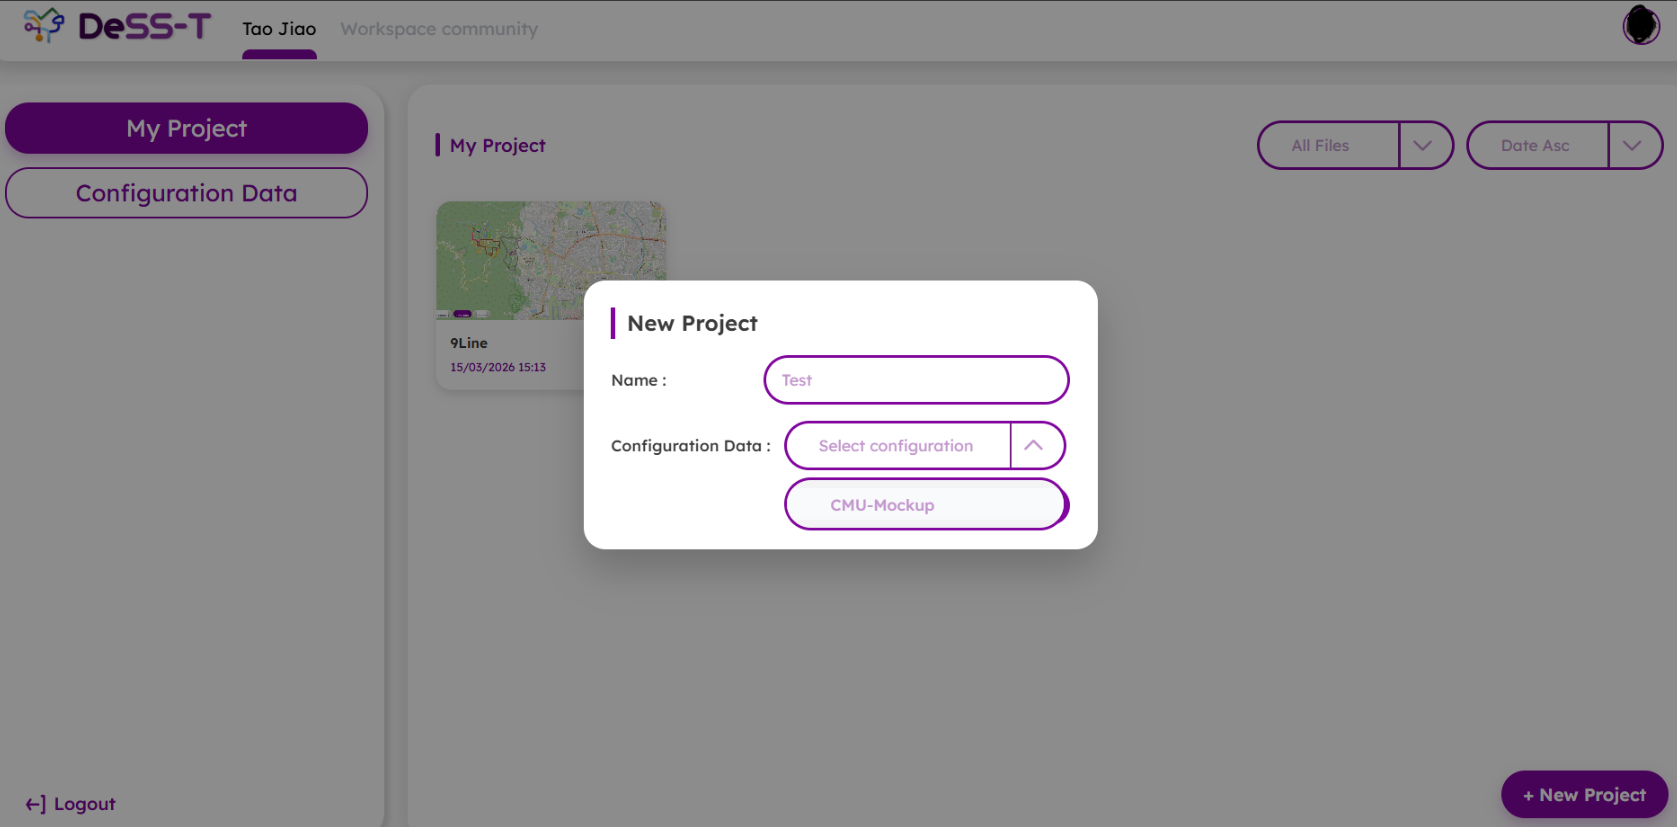
\includegraphics[scale=0.3]{3-5Pic/NewProject.png}
        \caption{หน้า New Project}
        \label{fig:WireframeNewWork}
      \end{figure}

    \item Step 3: การสร้างข้อมูล Configuration data ดังนี้
    \begin{itemize}
        \item ผู้ใช้สามารถสร้าง Configuration data ใหม่ได้ด้วยการกดที่ปุ่ม New Configuration และสามารถ Save Configuration 
        เพื่อใช้ในงานต่อไปได้ ตามภาพ \ref{fig:WireframeNewConfigLogin} และ \ref{fig:WireframeSetupConfigLogin}
          \begin{figure}[H]
            \centering
            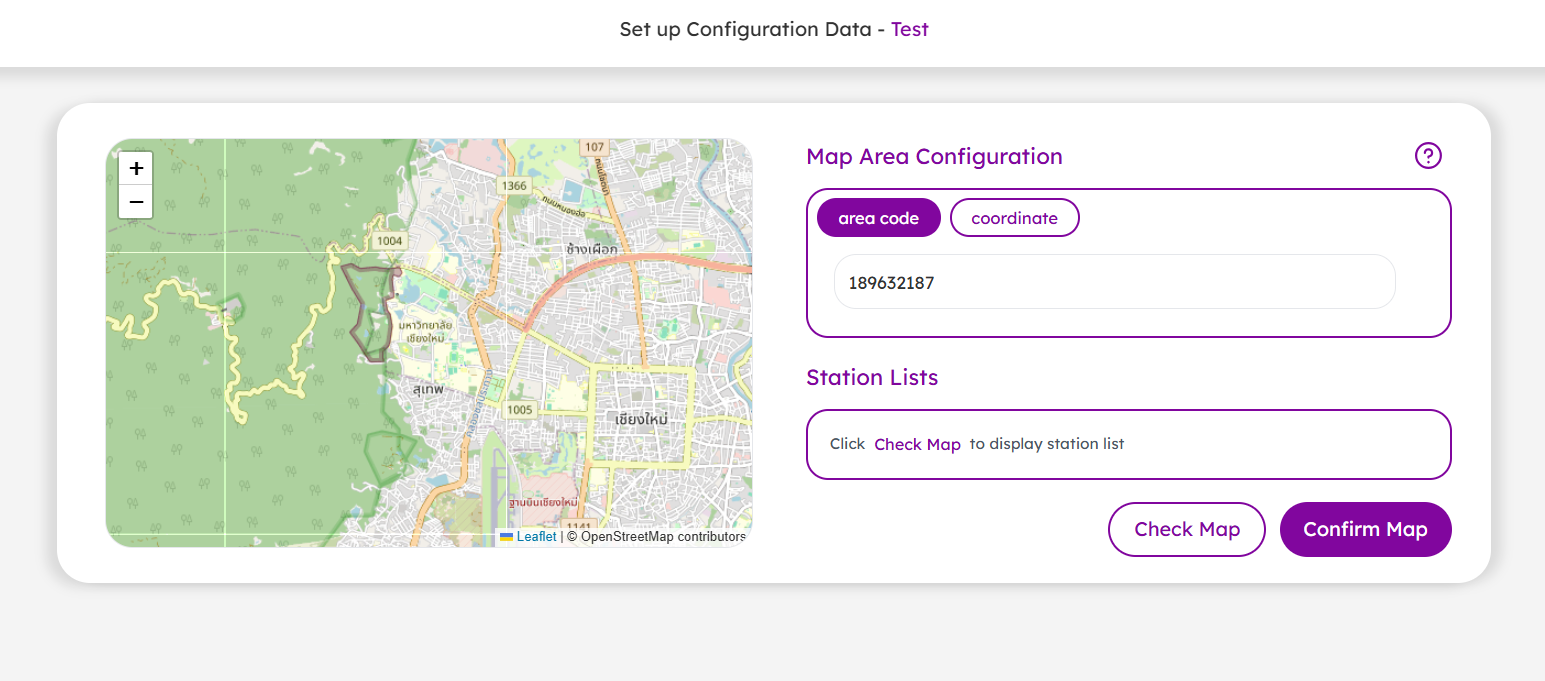
\includegraphics[scale=0.35]{3-5Pic/MapArea.png}
            \caption{หน้า New Configuration data สำหรับผู้ใช้ที่ลงทะเบียน}
            \label{fig:WireframeNewConfigLogin}
          \end{figure}

          \begin{figure}[H]
            \centering
            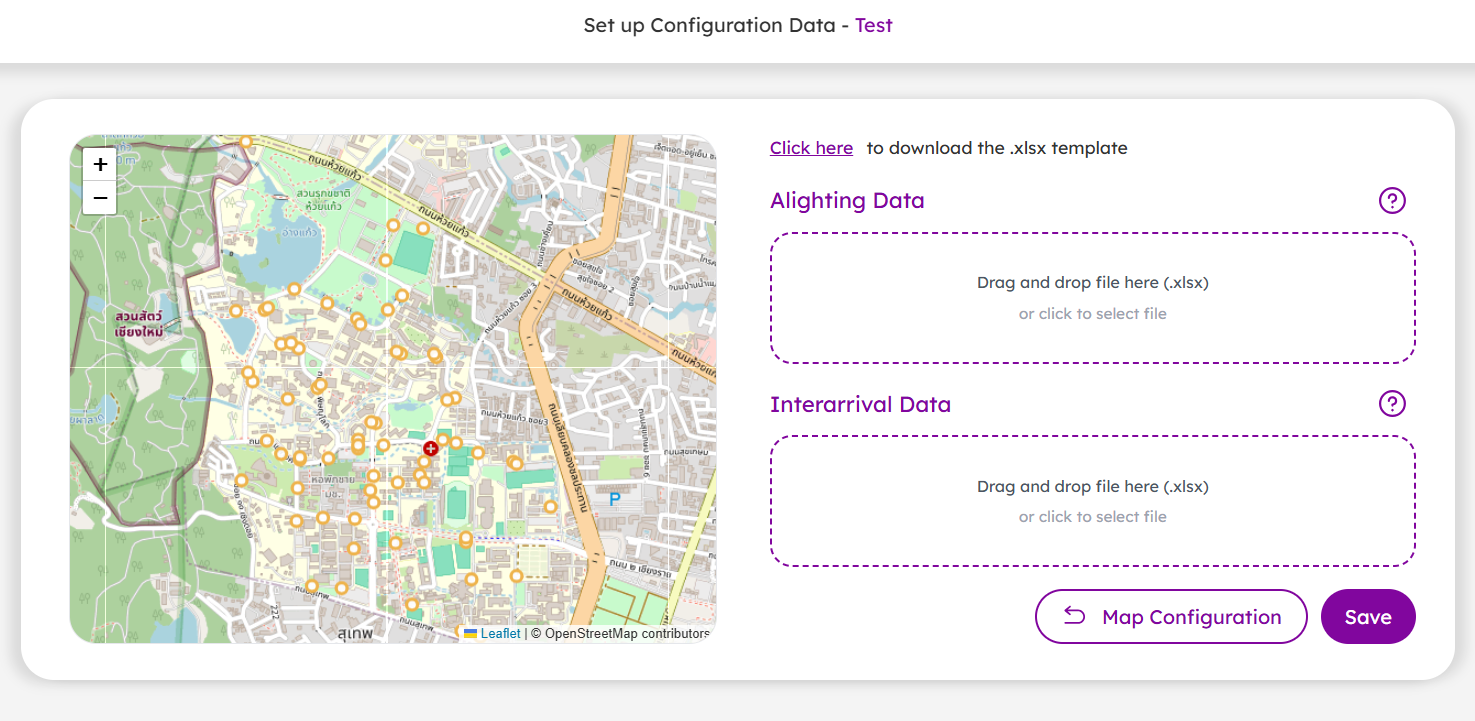
\includegraphics[scale=0.35]{3-5Pic/SetupConfigData.png}
            \caption{หน้า Setup Configuration data สำหรับผู้ใช้ที่ลงทะเบียน}
            \label{fig:WireframeSetupConfigLogin}
          \end{figure}

    \end{itemize}

    \item Step 4: หน้า Input Scenario page เพื่อกรอกข้อมูลสำหรับการจำลองบน Scenario ต่างๆ 
    ตามภาพ \ref{fig:WireframeInputLogin} และ \ref{fig:WireframeInputRouteLogin}
      \begin{figure}[H]
        \centering 
        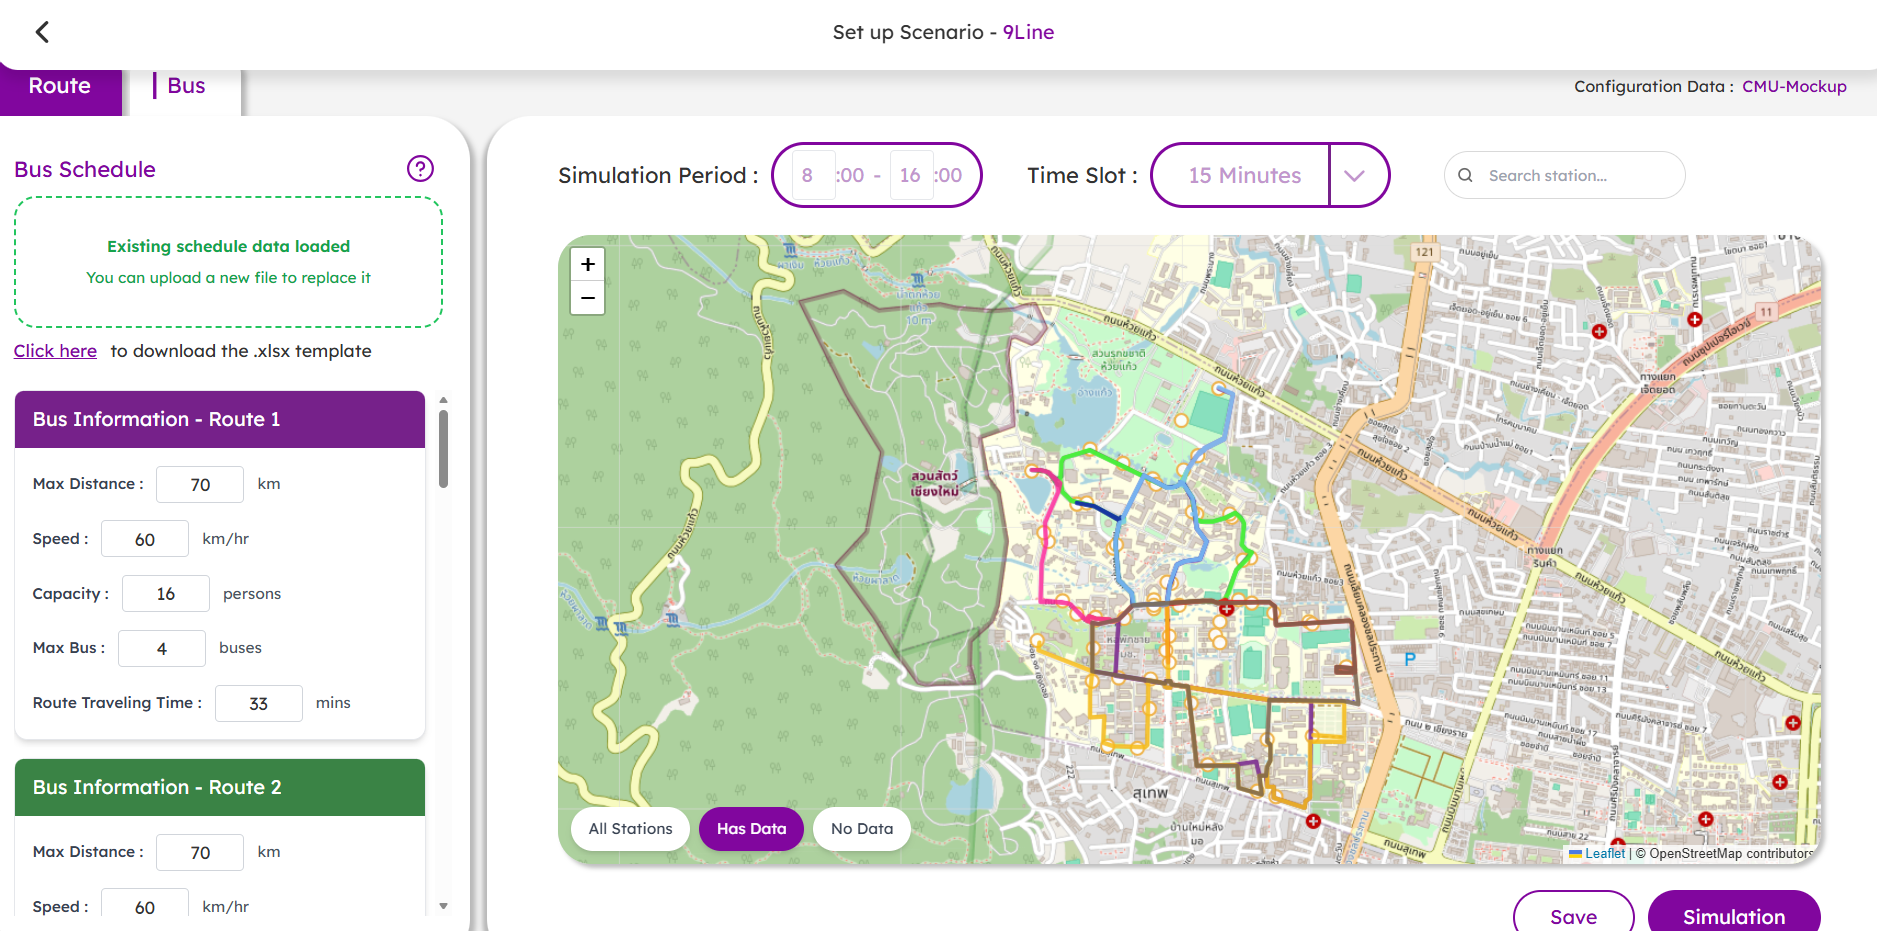
\includegraphics[scale=0.3]{3-5Pic/ScenarioBus.png}
        \caption{หน้า Input Scenario page (bus) }
        \label{fig:WireframeInputLogin}
      \end{figure}

      \begin{figure}[H]
        \centering
        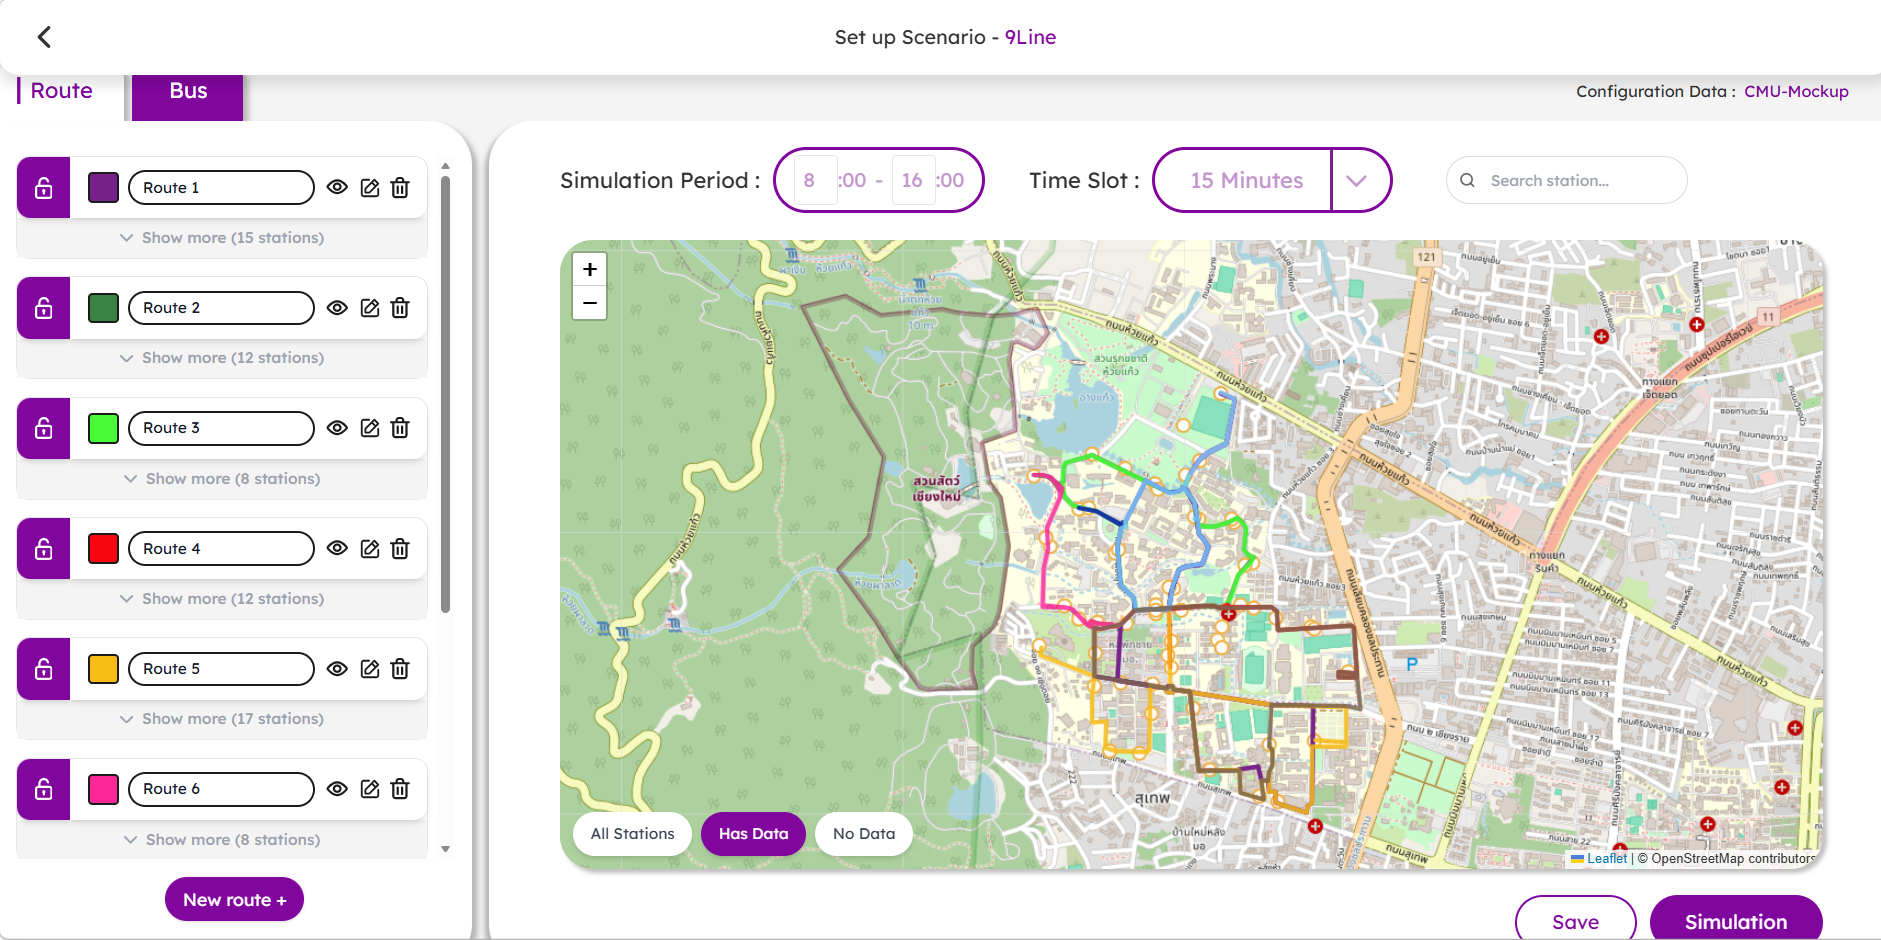
\includegraphics[scale=0.3]{3-5Pic/ScenarioRoute.png}
        \caption{หน้า Input Scenario page (route) }
        \label{fig:WireframeInputRouteLogin}
      \end{figure}

    \item Step 5: หลังจากผู้ใช้กดปุ่ม Run simulation แล้ว User จะสามารถเลือกดู  Dashboard สรุปผลข้อมูล 
    ตามภาพ \ref{fig:WireframeOutputLogin} และ \ref{fig:WireframeDashboardLogin}
      \begin{figure}[H]
        \centering
        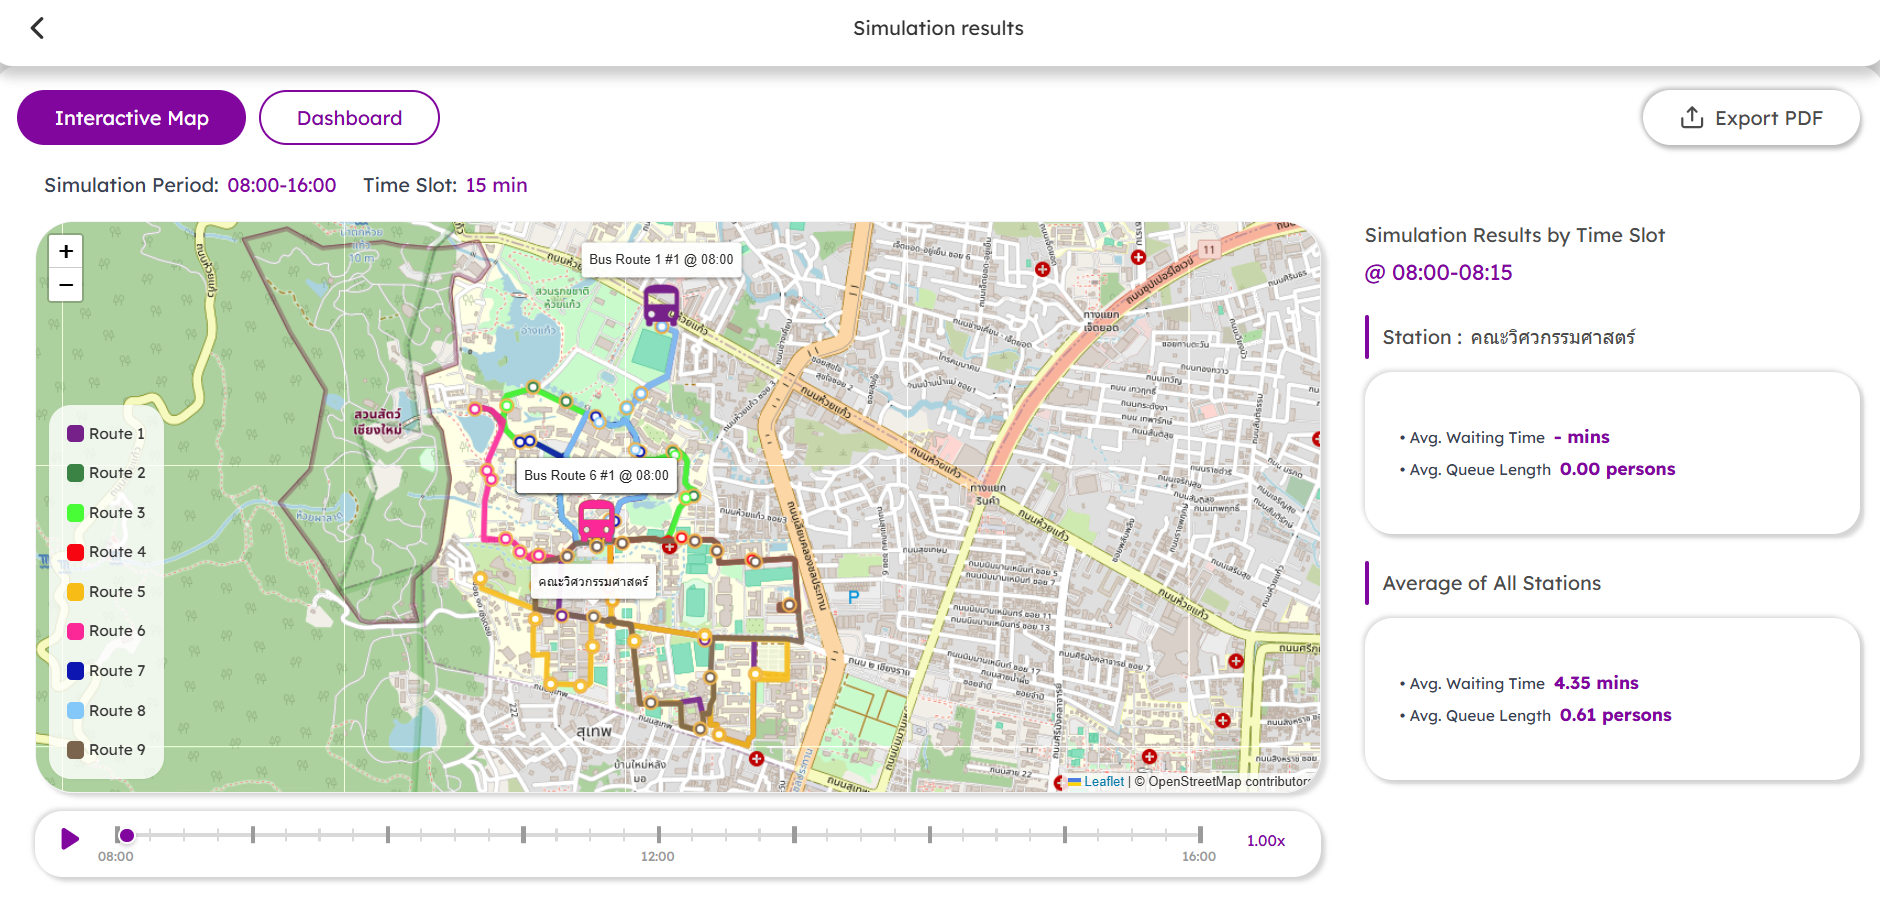
\includegraphics[scale=0.3]{3-5Pic/InteractiveMap.png}
        \caption{หน้าแสดงผลลัพธ์หลังจาก Run simulation}
        \label{fig:WireframeOutputLogin}
      \end{figure}

      \begin{figure}[H]
        \centering
        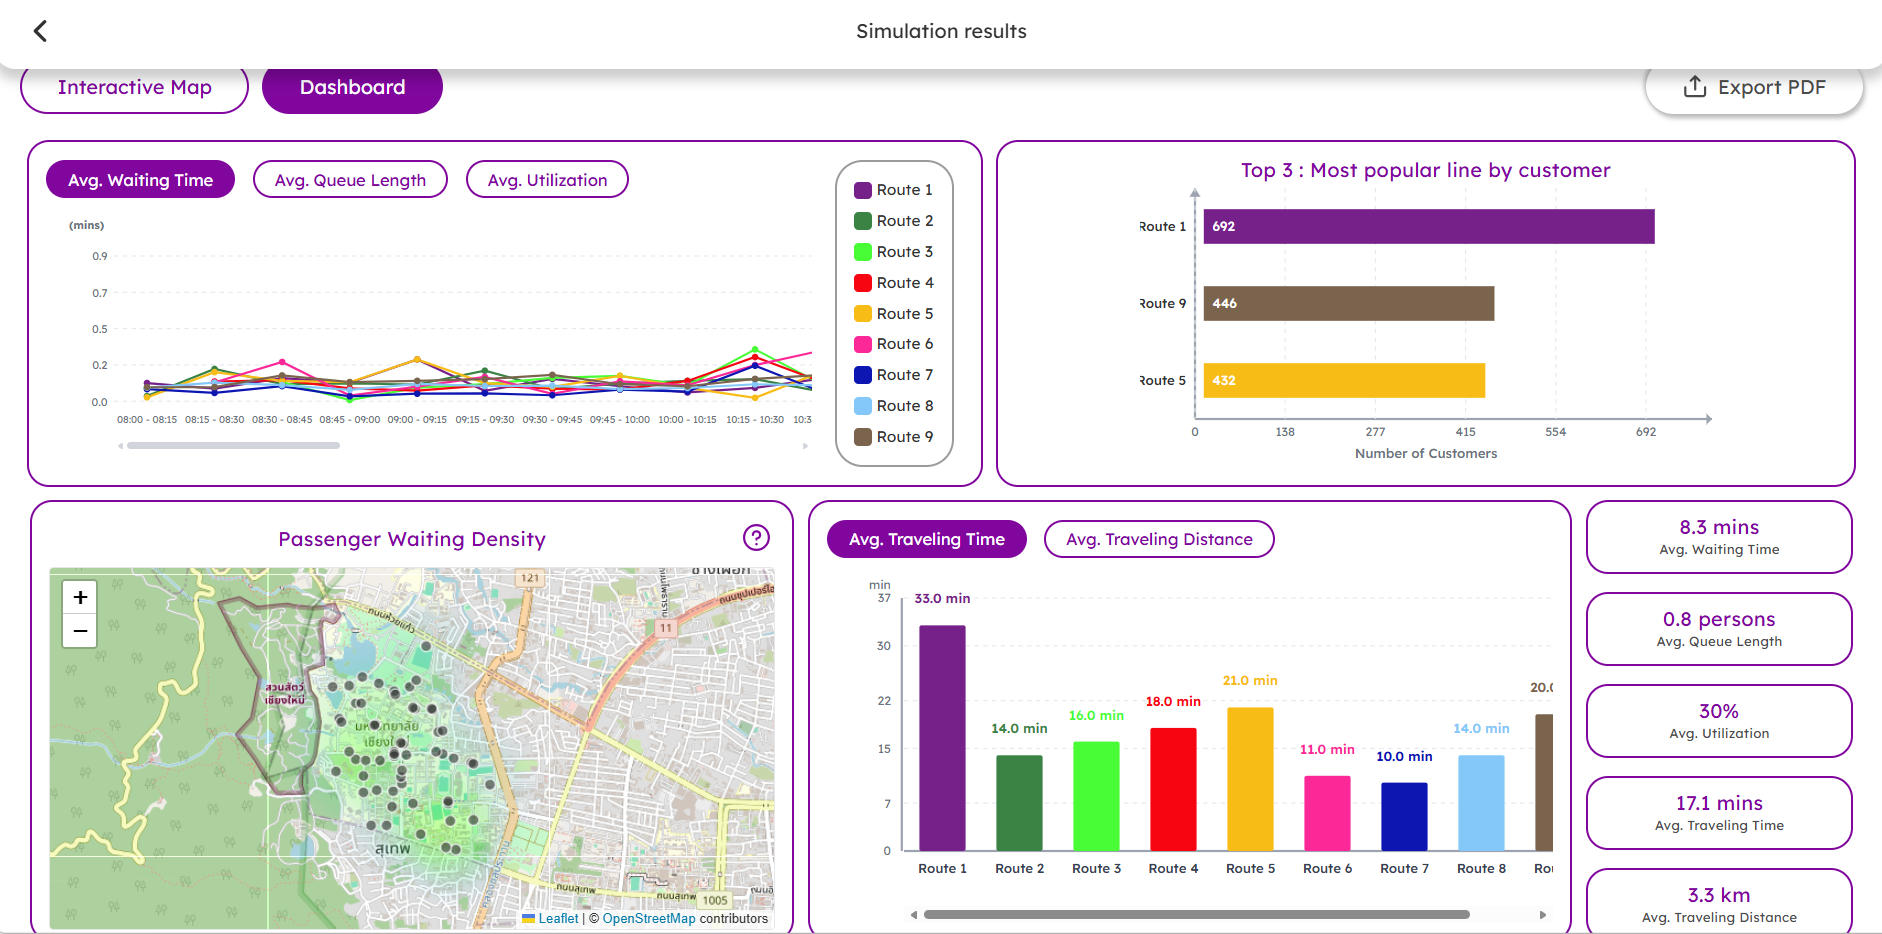
\includegraphics[scale=0.3]{3-5Pic/Dashboard.png} 
        \caption{หน้า Dashboard }
        \label{fig:WireframeDashboardLogin}
      \end{figure}

      \item Step 6: ผู้ใช้สามารถกด Export PDF เพื่อดูและบันทึกข้อมูลที่จำลองออกมาแบบละเอียดได้ 
      ตามภาพ \ref{fig:ExportPDFLogin}
      \begin{figure}[H]
        \centering
        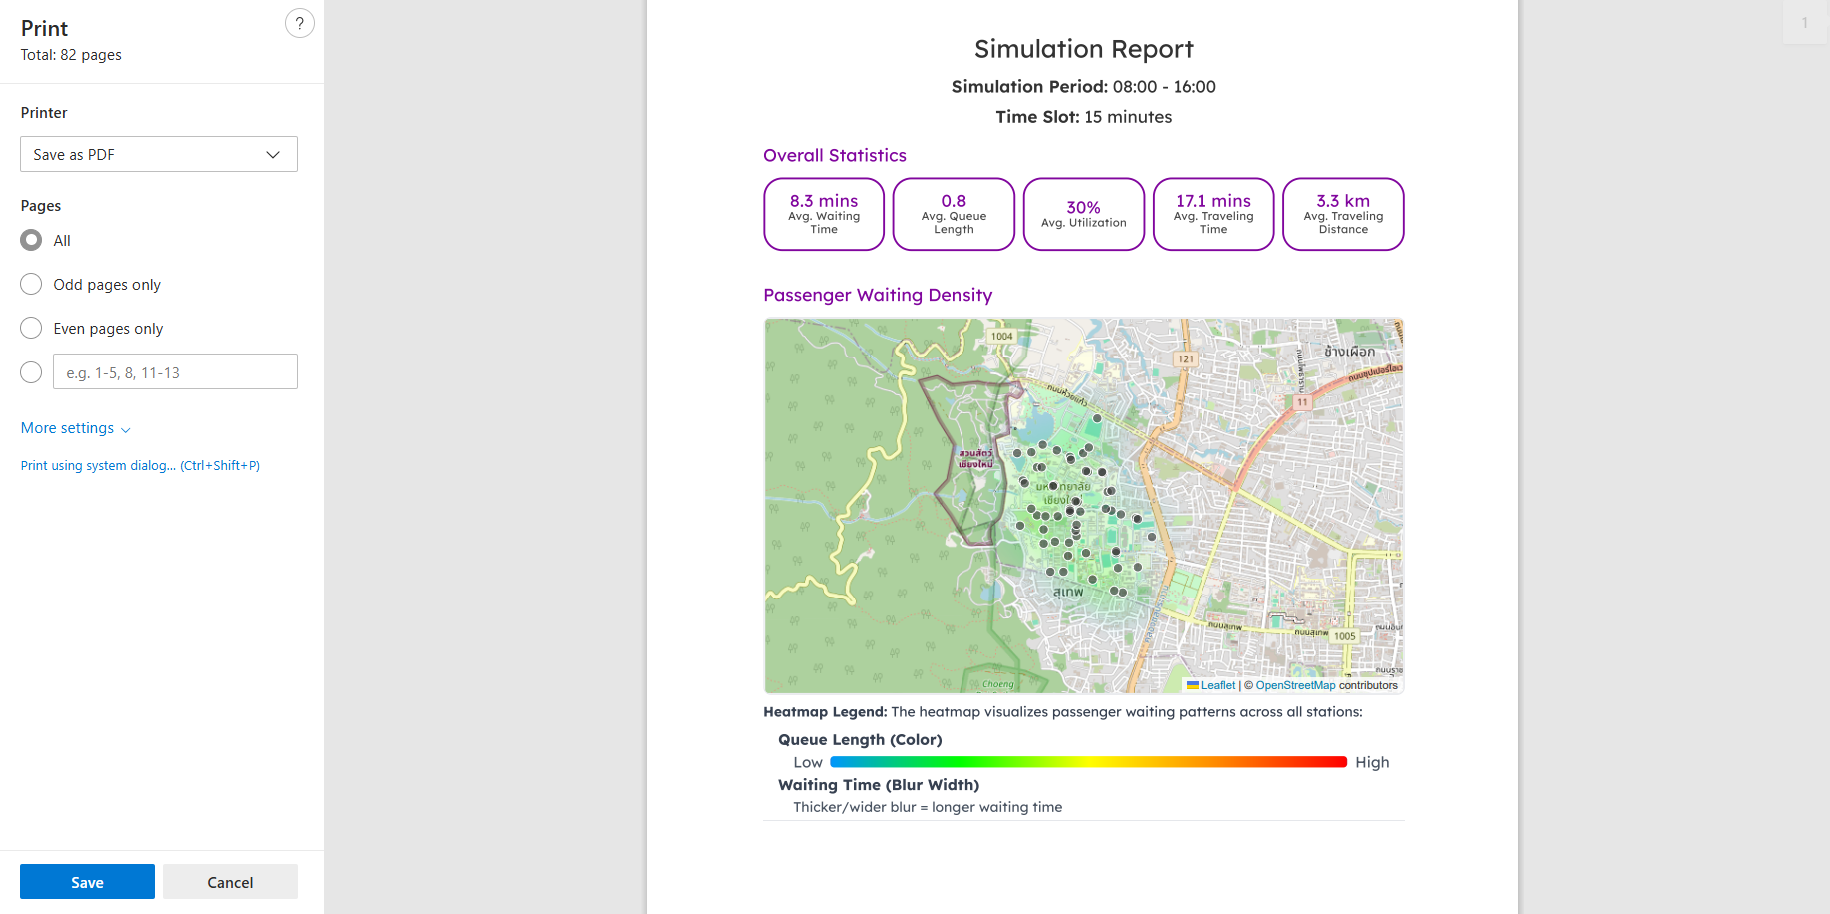
\includegraphics[scale=0.275]{3-5Pic/ExportPDFLOGIN.png}
        \caption{หน้า Export PDF}
        \label{fig:ExportPDFLogin}
      \end{figure}

    \end{itemize}
\end{mypara}

\section{รูปแบบไฟล์ข้อมูลนำเข้า (Supported Input File Formats)}
  \subsection{รูปแบบไฟล์ช่วงเวลาในการมาถึงของผู้โดยสาร (Passenger Arrival Time File Format)}
  \begin{mypara}
      \indent รูปแบบไฟล์ช่วงเวลาในการมาถึงของผู้โดยสาร ใช้สำหรับเก็บข้อมูลช่วงเวลาที่ผู้โดยสารแต่ละคนมาถึงที่สถานี
      โดยข้อมูลจะถูกจัดเก็บในไฟล์ Excel โดยมีสกุลไฟล์ \texttt{.xlsx} 
      ซึ่งมีโครงสร้างดังแสดงในภาพ \ref{fig:PassengerArrivalFileFormat}
      \begin{figure}[H]
        \centering
        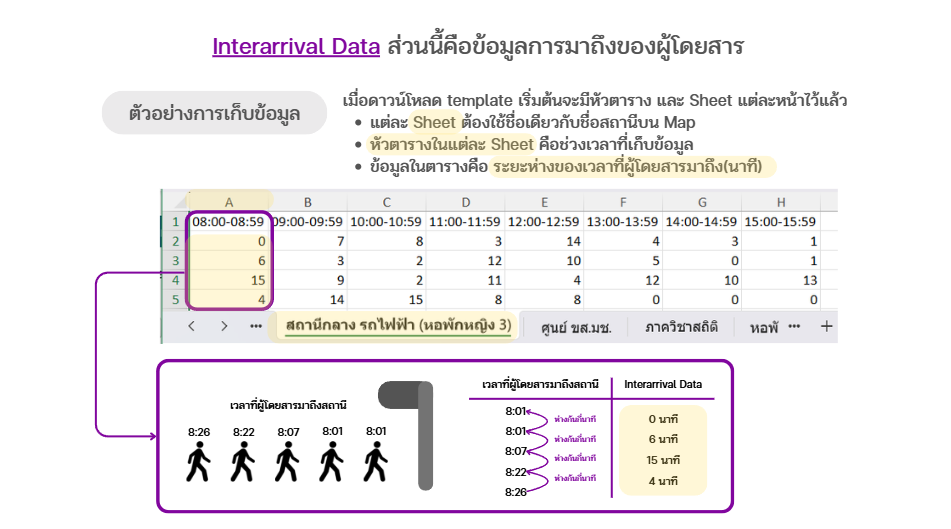
\includegraphics[scale=0.7]{Passenger_Interarrival.png}
        \caption{รูปแบบไฟล์ช่วงเวลาในการมาถึงของผู้โดยสาร}
        \label{fig:PassengerArrivalFileFormat}
      \end{figure}
  \end{mypara}

  \newpage
  \subsection{รูปแบบไฟล์จำนวนผู้โดยสารที่ลงจากรถ (Passenger Alight File Format)}
  \begin{mypara}
      \indent รูปแบบไฟล์จำนวนผู้โดยสารที่ลงจากรถ ใช้สำหรับเก็บข้อมูลจำนวนผู้โดยสารที่ลงจากรถในแต่ละสถานี
      โดยข้อมูลจะถูกจัดเก็บในไฟล์ Excel โดยมีสกุลไฟล์ \texttt{.xlsx} 
      ซึ่งมีโครงสร้างดังแสดงในภาพ \ref{fig:PassengerAlightFileFormat}
      \begin{figure}[H]
        \centering
        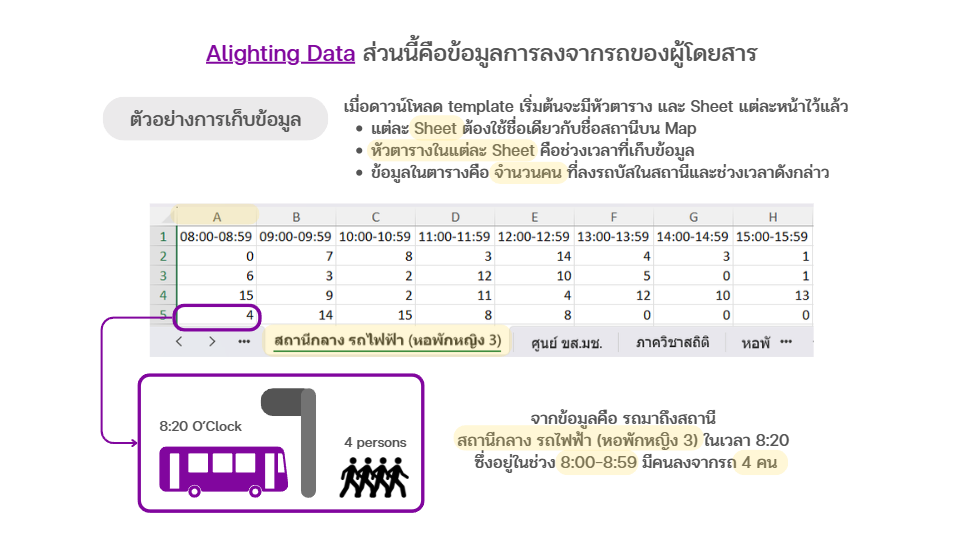
\includegraphics[scale=0.7]{Passenger_alighting.png}
        \caption{รูปแบบไฟล์จำนวนผู้โดยสารที่ลงจากรถ}
        \label{fig:PassengerAlightFileFormat}
      \end{figure}
  \end{mypara}

  \subsection{รูปแบบไฟล์ตารางการเดินรถ (Bus Schedule File Format)}
  \begin{mypara}
      \indent รูปแบบไฟล์ตารางการเดินรถ ใช้สำหรับเก็บข้อมูลเวลาการออกรถของแต่ละสายบริการ 
      โดยข้อมูลจะถูกจัดเก็บในไฟล์ Excel โดยมีสกุลไฟล์ \texttt{.xlsx} 
      ซึ่งมีโครงสร้างดังแสดงในภาพ \ref{fig:BusScheduleFileFormat}
      \begin{figure}[H]
        \centering
        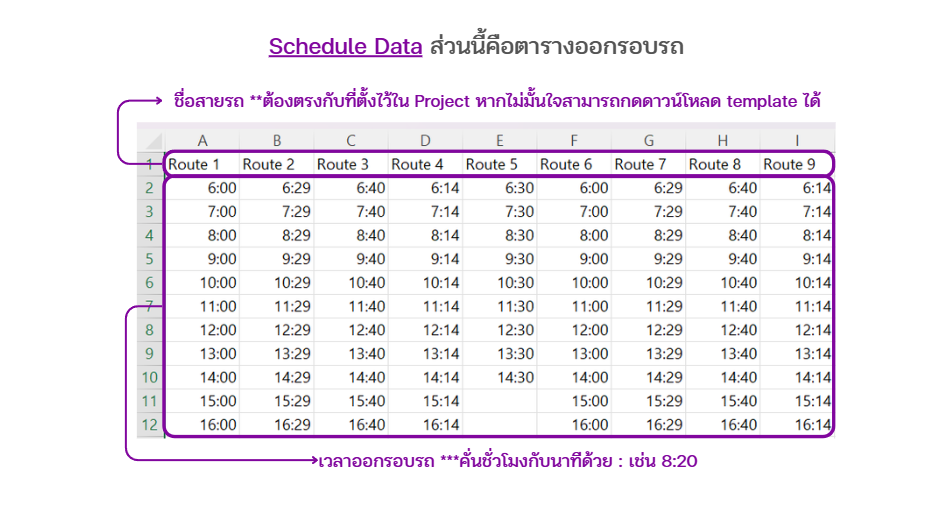
\includegraphics[scale=0.7]{bus_schedule.png}
        \caption{รูปแบบไฟล์ตารางการเดินรถ}
        \label{fig:BusScheduleFileFormat}
      \end{figure}
  \end{mypara}